\documentclass[12pt,a4paper,landscape]{article}
\usepackage[utf8]{inputenc}
\usepackage[T1]{fontenc}
\usepackage{graphicx}
\usepackage{booktabs}
\usepackage[margin=0.5in, top=0.5in, headsep=0.1in]{geometry}
\usepackage{caption}
\usepackage{float}
\usepackage[authoryear,round]{natbib}
\usepackage{xcolor}
\usepackage{colortbl}
\usepackage{rotating}
\usepackage{tabularx}
\usepackage{pdflscape}
\usepackage{adjustbox}
\usepackage{times}
\usepackage{array}
\usepackage{fancyhdr}
\usepackage[colorlinks=true, allcolors=blue]{hyperref}

% Setup fancy headers
\fancypagestyle{mainStyle}{%
    \fancyhf{}
    \renewcommand{\headrulewidth}{0pt}
    \fancyhead[R]{\footnotesize\hyperref[toc]{Back to Contents}}
}

\pagestyle{mainStyle}

\newcommand{\countryheader}[2]{\large\bfseries\hyperref[#1]{#2}}
\captionsetup[table]{labelformat=empty}
\definecolor{lightgray}{gray}{0.85}

\begin{document}
\title{\Large Country Data and Graphs for Ireland}
\date{June 30, 2025}
\maketitle
\thispagestyle{empty}

\clearpage
\setcounter{page}{1}
\hypersetup{colorlinks=true,linkcolor=blue,linktoc=all}
\phantomsection
\label{toc}
\tableofcontents
\thispagestyle{empty}
\clearpage
\phantomsection
\addcontentsline{toc}{section}{Data availability heatmap}
\begin{center}
{\Large\bfseries Data availability heatmap}
\end{center}
\vspace{1cm}
\begin{figure}[H]
\centering
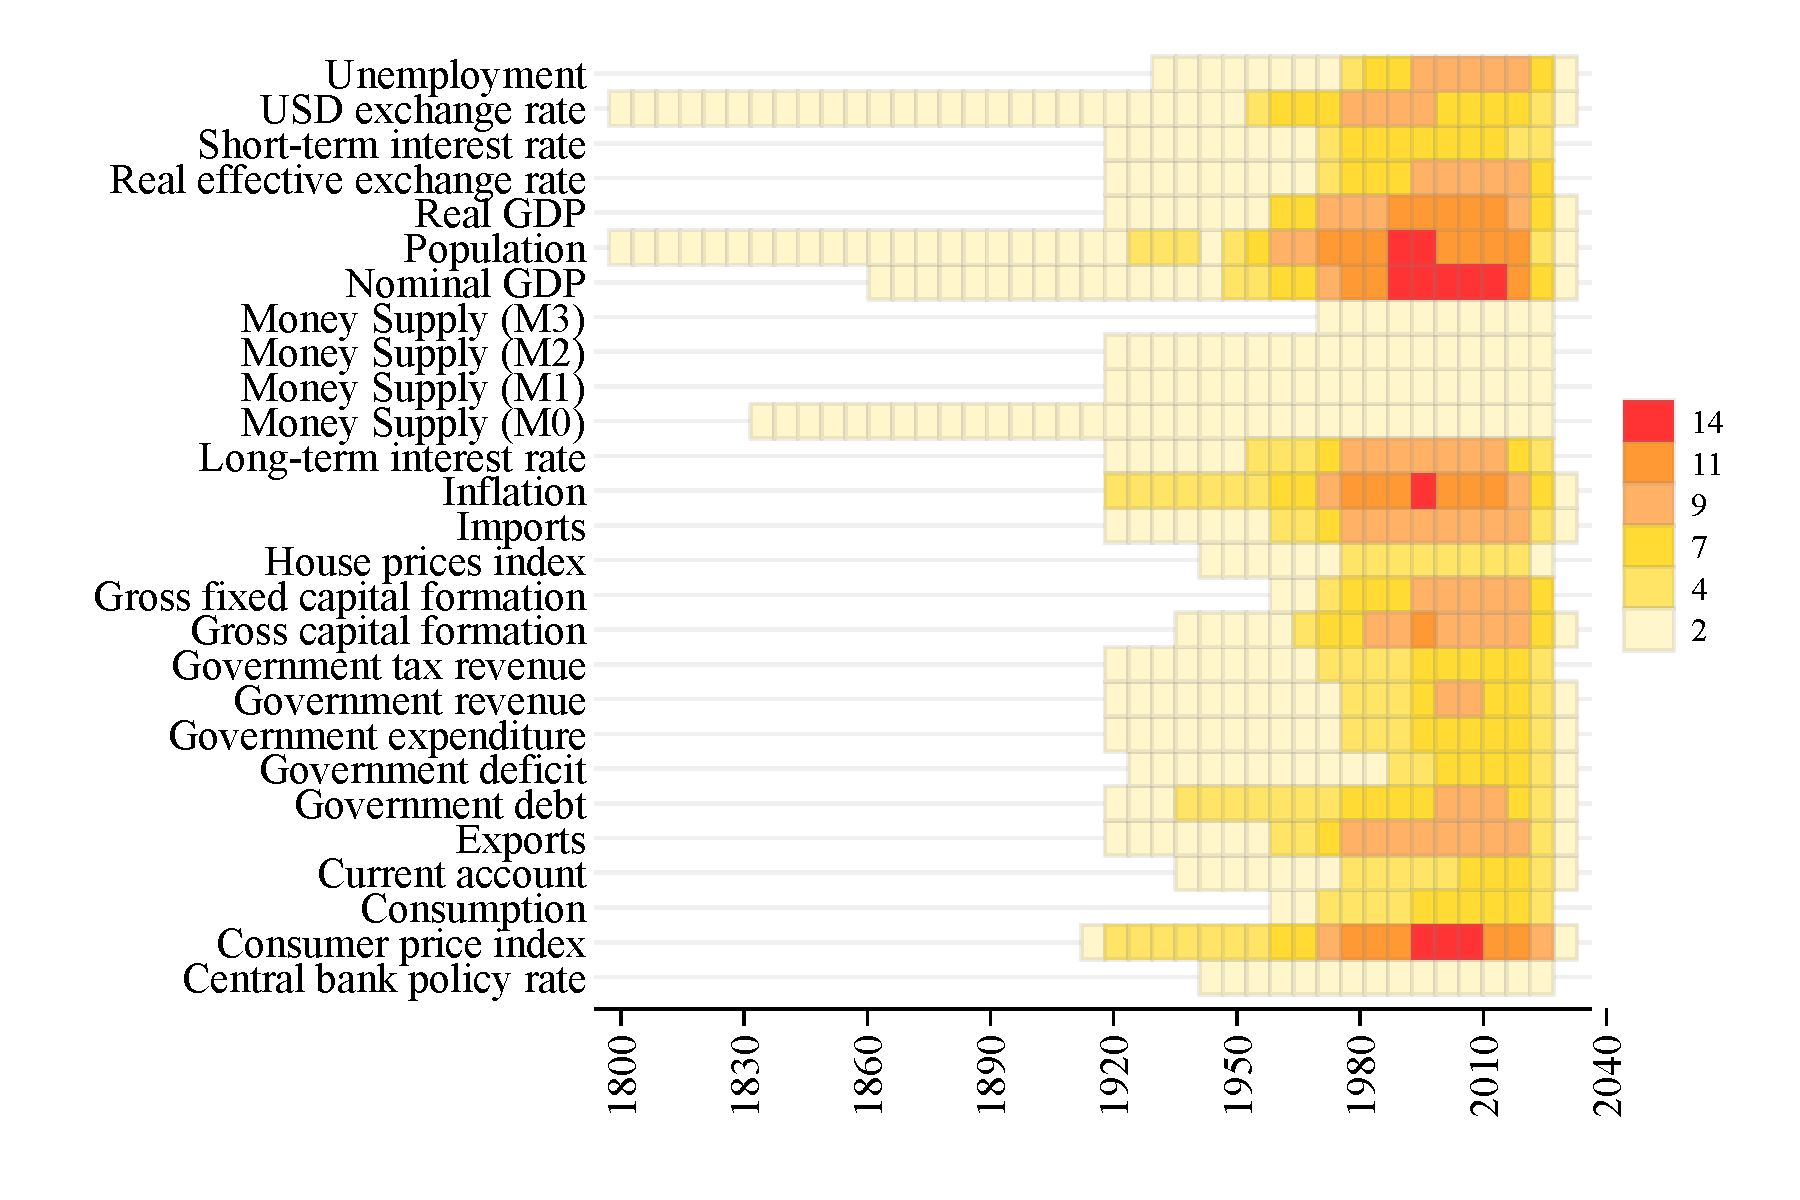
\includegraphics[width=\textwidth,height=0.8\textheight,keepaspectratio]{graphs/IRL_heatmap.pdf}
\end{figure}
\setcounter{page}{3}
\begin{adjustbox}{max totalsize={\paperwidth}{\paperheight},center}
\begin{minipage}[t][\textheight][t]{\textwidth}
\vspace*{0.5cm}
\phantomsection
\addcontentsline{toc}{section}{Current account balance}
\begin{center}
{\Large\bfseries Current account balance}
\end{center}
\vspace{0.5cm}
\begin{table}[H]
\centering
\small
\begin{tabular}{|l|l|l|}
\hline
\textbf{Source} & \textbf{Time span} & \textbf{Notes} \\
\hline
\rowcolor{white}\cite{JST}& 1938 - 1973 &Spliced using overlapping data in 1974. \\
\rowcolor{lightgray}\cite{WDI_ARC}& 1974 - 1989 &Spliced using overlapping data in 1990. \\
\rowcolor{white}\cite{OECD_EO}& 1990 - 2025 &Baseline source, overlaps with base year 2018. \\
\rowcolor{lightgray}\cite{IMF_WEO_forecast}& 2026 - 2029 &Spliced using overlapping data in 2030. \\
\hline
\end{tabular}
\end{table}
\begin{figure}[H]
\centering
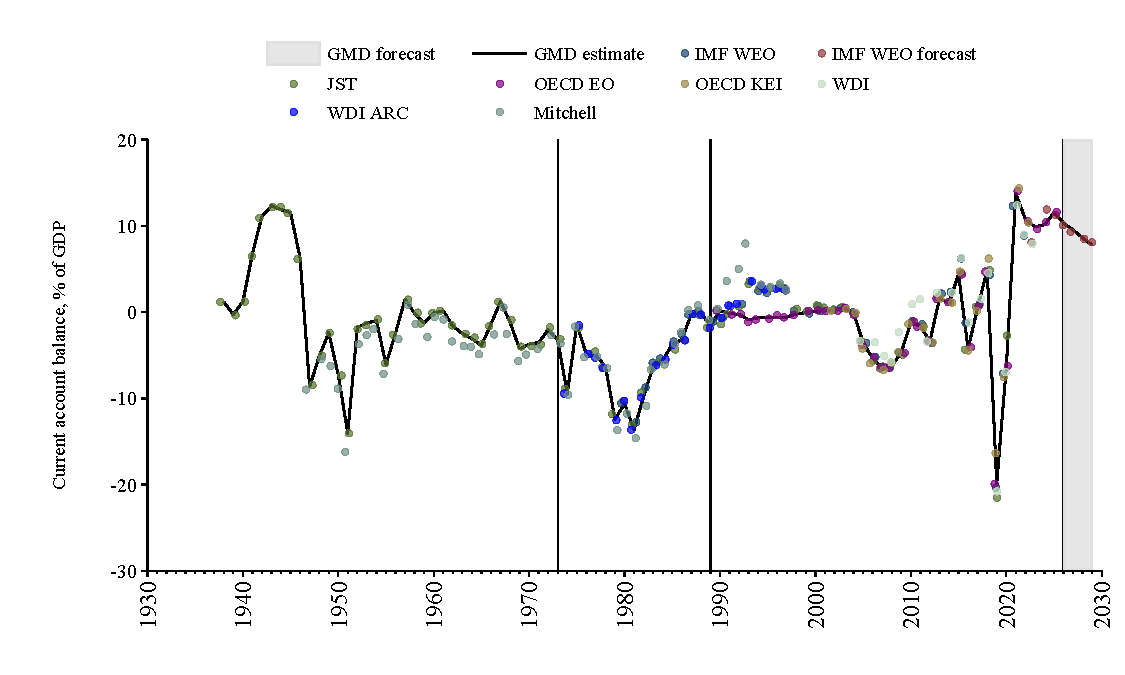
\includegraphics[width=\textwidth,height=0.6\textheight,keepaspectratio]{graphs/IRL_CA_GDP.pdf}
\end{figure}
\end{minipage}
\end{adjustbox}
\begin{adjustbox}{max totalsize={\paperwidth}{\paperheight},center}
\begin{minipage}[t][\textheight][t]{\textwidth}
\vspace*{0.5cm}
\phantomsection
\addcontentsline{toc}{section}{Consumer price index}
\begin{center}
{\Large\bfseries Consumer price index}
\end{center}
\vspace{0.5cm}
\begin{table}[H]
\centering
\small
\begin{tabular}{|l|l|l|}
\hline
\textbf{Source} & \textbf{Time span} & \textbf{Notes} \\
\hline
\rowcolor{white}\cite{HFS}& 1914 - 1914 &Spliced using overlapping data in 1915. \\
\rowcolor{lightgray}\cite{BIS}& 1915 - 2024 &Baseline source, overlaps with base year 2018. \\
\rowcolor{white}\cite{OECD_EO}& 2025 - 2025 &Spliced using overlapping data in 2026: (ratio = 109.7\%). \\
\rowcolor{lightgray}\cite{AMECO}& 2026 - 2026 &Spliced using overlapping data in 2027: (ratio = 104.7\%). \\
\rowcolor{white}\cite{IMF_WEO_forecast}& 2027 - 2029 &Spliced using overlapping data in 2030: (ratio = 106.3\%). \\
\hline
\end{tabular}
\end{table}
\begin{figure}[H]
\centering
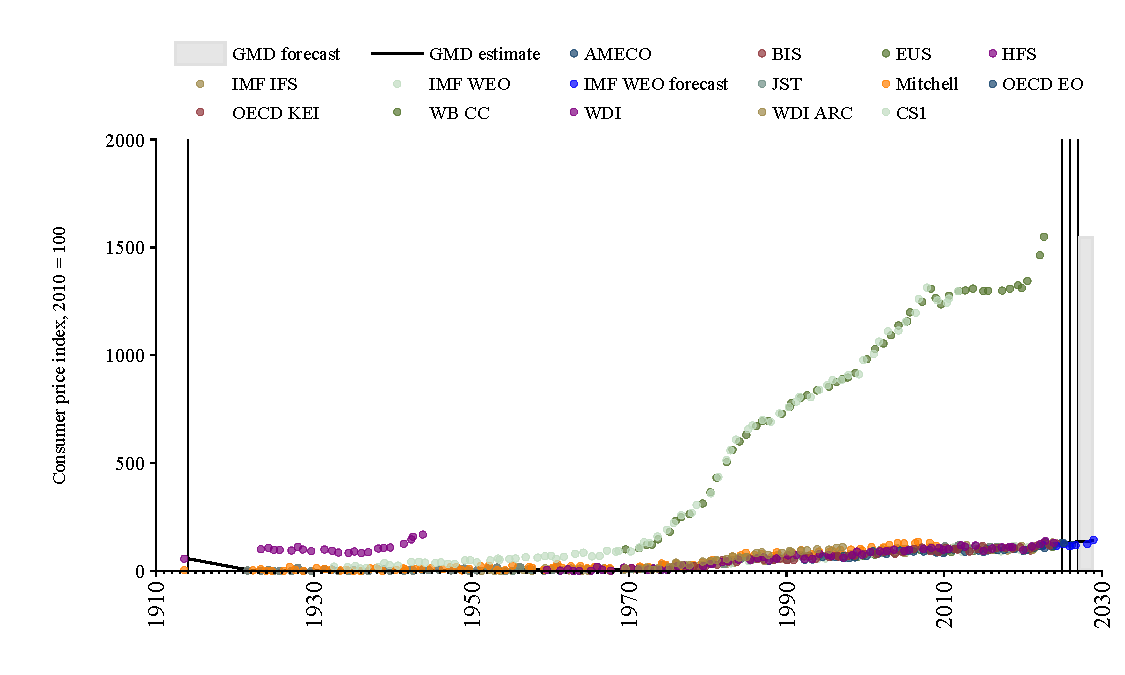
\includegraphics[width=\textwidth,height=0.6\textheight,keepaspectratio]{graphs/IRL_CPI.pdf}
\end{figure}
\end{minipage}
\end{adjustbox}
\begin{adjustbox}{max totalsize={\paperwidth}{\paperheight},center}
\begin{minipage}[t][\textheight][t]{\textwidth}
\vspace*{0.5cm}
\phantomsection
\addcontentsline{toc}{section}{House price index}
\begin{center}
{\Large\bfseries House price index}
\end{center}
\vspace{0.5cm}
\begin{table}[H]
\centering
\small
\begin{tabular}{|l|l|l|}
\hline
\textbf{Source} & \textbf{Time span} & \textbf{Notes} \\
\hline
\rowcolor{white}\cite{JST}& 1945 - 1969 &Spliced using overlapping data in 1970. \\
\rowcolor{lightgray}\cite{BIS}& 1970 - 2025 &Baseline source, overlaps with base year 2018. \\
\hline
\end{tabular}
\end{table}
\begin{figure}[H]
\centering
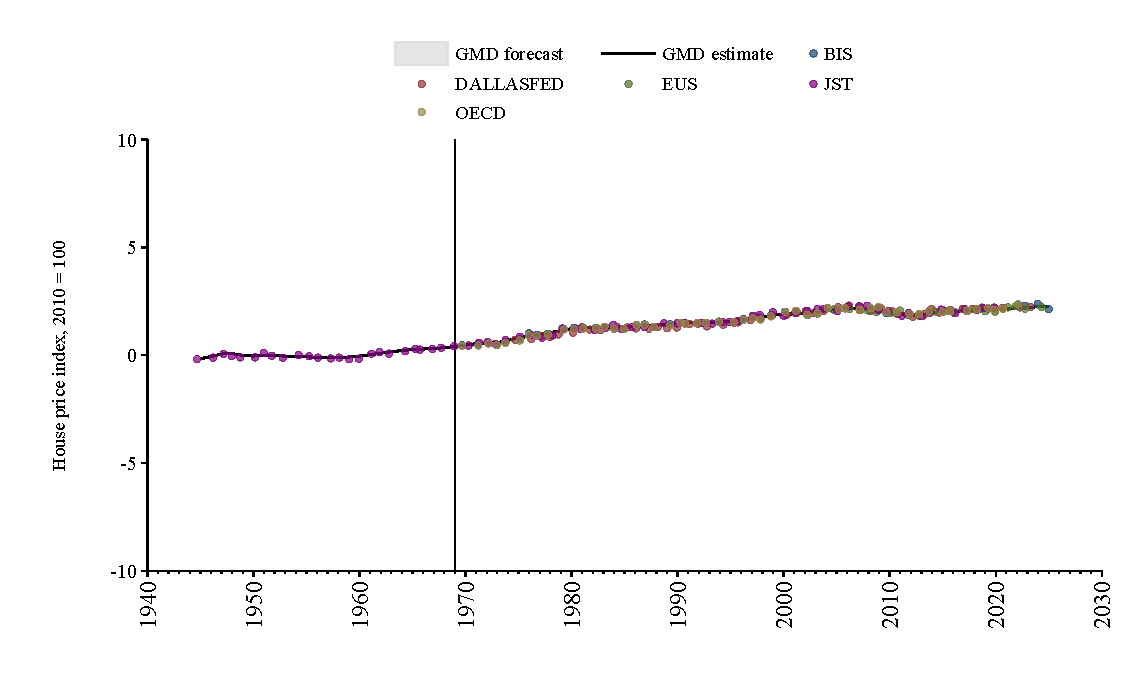
\includegraphics[width=\textwidth,height=0.6\textheight,keepaspectratio]{graphs/IRL_HPI.pdf}
\end{figure}
\end{minipage}
\end{adjustbox}
\begin{adjustbox}{max totalsize={\paperwidth}{\paperheight},center}
\begin{minipage}[t][\textheight][t]{\textwidth}
\vspace*{0.5cm}
\phantomsection
\addcontentsline{toc}{section}{Money supply (M0)}
\begin{center}
{\Large\bfseries Money supply (M0)}
\end{center}
\vspace{0.5cm}
\begin{table}[H]
\centering
\small
\begin{tabular}{|l|l|l|}
\hline
\textbf{Source} & \textbf{Time span} & \textbf{Notes} \\
\hline
\rowcolor{white}\cite{Mitchell}& 1833 - 2010 &Spliced using overlapping data in 2011. \\
\hline
\end{tabular}
\end{table}
\begin{figure}[H]
\centering
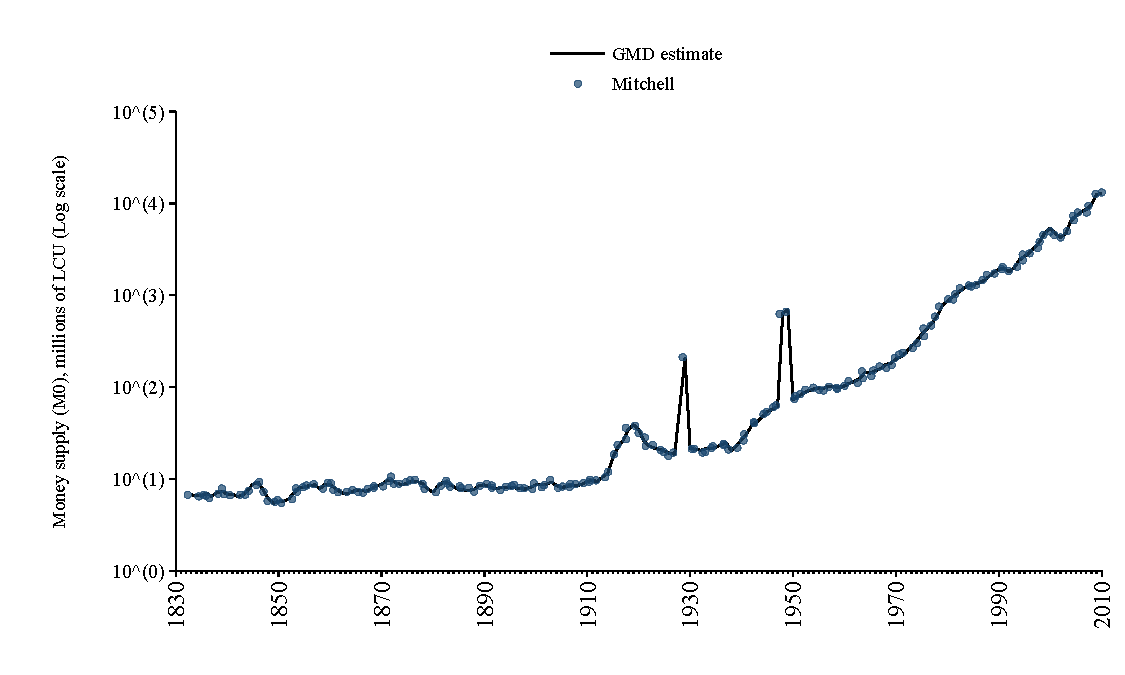
\includegraphics[width=\textwidth,height=0.6\textheight,keepaspectratio]{graphs/IRL_M0.pdf}
\end{figure}
\end{minipage}
\end{adjustbox}
\begin{adjustbox}{max totalsize={\paperwidth}{\paperheight},center}
\begin{minipage}[t][\textheight][t]{\textwidth}
\vspace*{0.5cm}
\phantomsection
\addcontentsline{toc}{section}{Money supply (M1)}
\begin{center}
{\Large\bfseries Money supply (M1)}
\end{center}
\vspace{0.5cm}
\begin{table}[H]
\centering
\small
\begin{tabular}{|l|l|l|}
\hline
\textbf{Source} & \textbf{Time span} & \textbf{Notes} \\
\hline
\rowcolor{white}\cite{JST}& 1922 - 2020 &Baseline source, overlaps with base year 2018. \\
\hline
\end{tabular}
\end{table}
\begin{figure}[H]
\centering
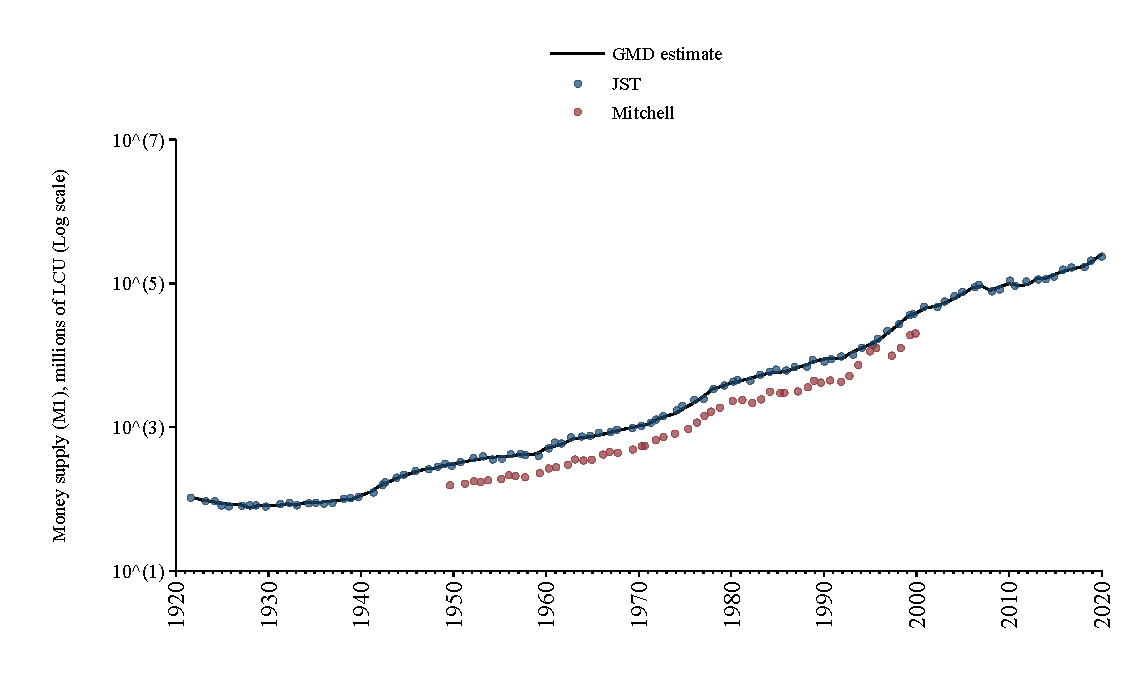
\includegraphics[width=\textwidth,height=0.6\textheight,keepaspectratio]{graphs/IRL_M1.pdf}
\end{figure}
\end{minipage}
\end{adjustbox}
\begin{adjustbox}{max totalsize={\paperwidth}{\paperheight},center}
\begin{minipage}[t][\textheight][t]{\textwidth}
\vspace*{0.5cm}
\phantomsection
\addcontentsline{toc}{section}{Money supply (M2)}
\begin{center}
{\Large\bfseries Money supply (M2)}
\end{center}
\vspace{0.5cm}
\begin{table}[H]
\centering
\small
\begin{tabular}{|l|l|l|}
\hline
\textbf{Source} & \textbf{Time span} & \textbf{Notes} \\
\hline
\rowcolor{white}\cite{JST}& 1922 - 2020 &Baseline source, overlaps with base year 2018. \\
\hline
\end{tabular}
\end{table}
\begin{figure}[H]
\centering
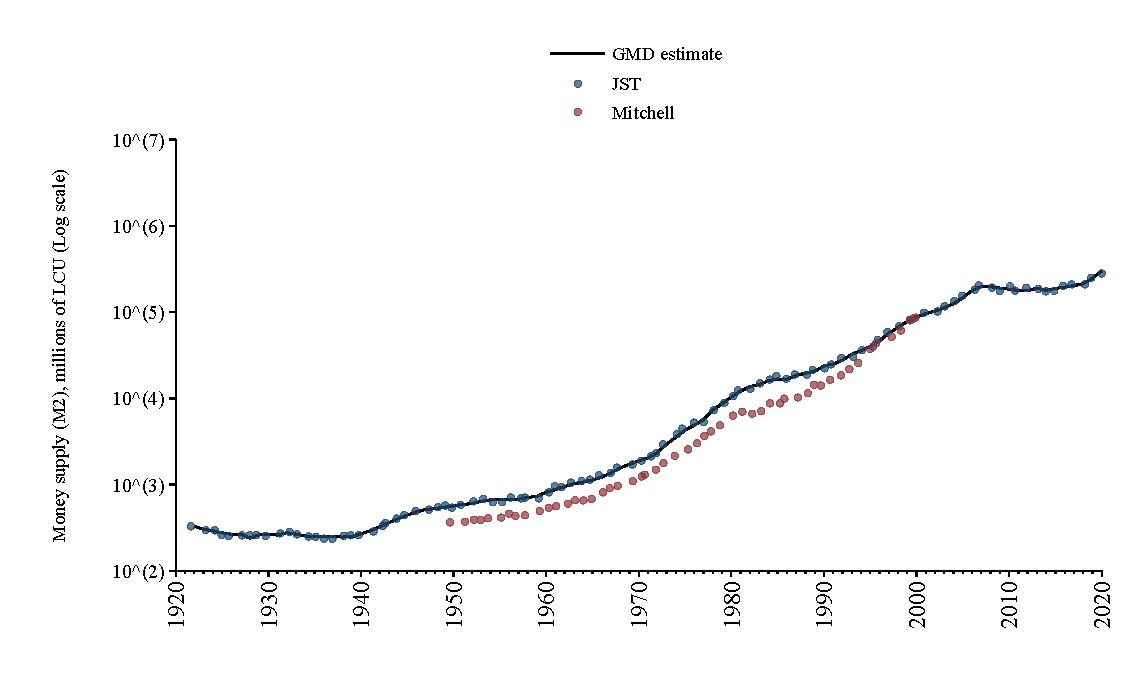
\includegraphics[width=\textwidth,height=0.6\textheight,keepaspectratio]{graphs/IRL_M2.pdf}
\end{figure}
\end{minipage}
\end{adjustbox}
\begin{adjustbox}{max totalsize={\paperwidth}{\paperheight},center}
\begin{minipage}[t][\textheight][t]{\textwidth}
\vspace*{0.5cm}
\phantomsection
\addcontentsline{toc}{section}{Real effective exchange rate}
\begin{center}
{\Large\bfseries Real effective exchange rate}
\end{center}
\vspace{0.5cm}
\begin{table}[H]
\centering
\small
\begin{tabular}{|l|l|l|}
\hline
\textbf{Source} & \textbf{Time span} & \textbf{Notes} \\
\hline
\rowcolor{white}\cite{LUND}& 1923 - 1959 &Spliced using overlapping data in 1960: (ratio = 101.8\%). \\
\rowcolor{lightgray}\cite{BRUEGEL}& 1960 - 1974 &Spliced using overlapping data in 1975: (ratio = 169.9\%). \\
\rowcolor{white}\cite{WDI_ARC}& 1975 - 1978 &Spliced using overlapping data in 1979: (ratio = 94.7\%). \\
\rowcolor{lightgray}\cite{WDI}& 1979 - 2023 &Baseline source, overlaps with base year 2018. \\
\rowcolor{white}\cite{BIS}& 2024 - 2025 &Spliced using overlapping data in 2026: (ratio = 87.6\%). \\
\hline
\end{tabular}
\end{table}
\begin{figure}[H]
\centering
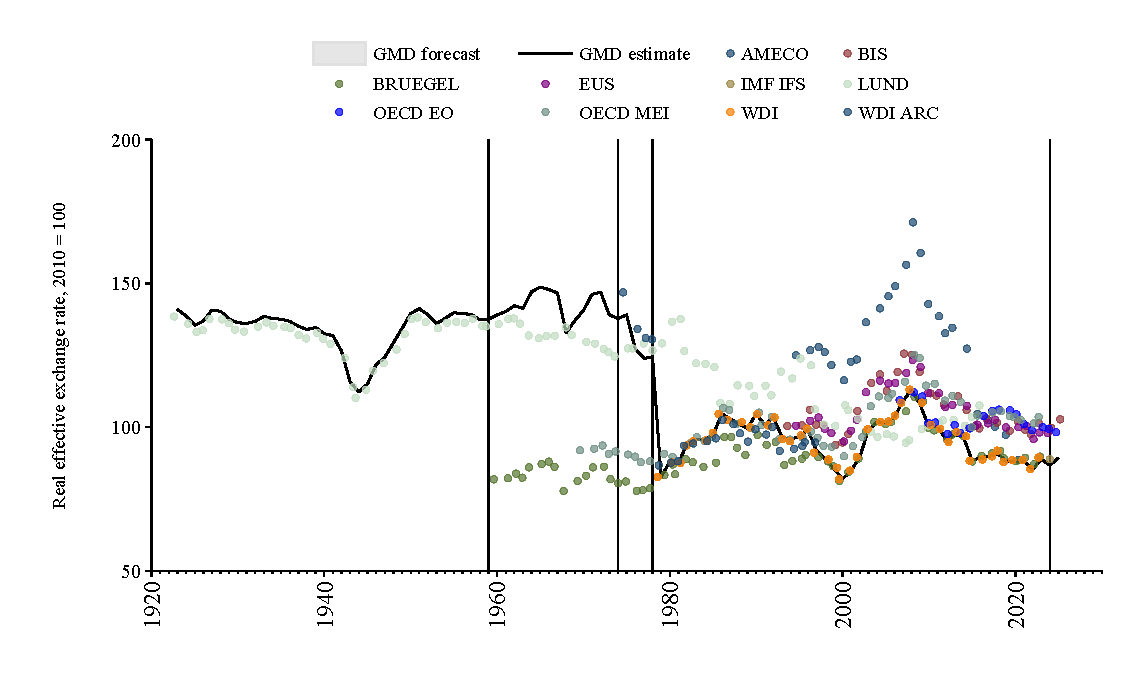
\includegraphics[width=\textwidth,height=0.6\textheight,keepaspectratio]{graphs/IRL_REER.pdf}
\end{figure}
\end{minipage}
\end{adjustbox}
\begin{adjustbox}{max totalsize={\paperwidth}{\paperheight},center}
\begin{minipage}[t][\textheight][t]{\textwidth}
\vspace*{0.5cm}
\phantomsection
\addcontentsline{toc}{section}{USD exchange rate}
\begin{center}
{\Large\bfseries USD exchange rate}
\end{center}
\vspace{0.5cm}
\begin{table}[H]
\centering
\small
\begin{tabular}{|l|l|l|}
\hline
\textbf{Source} & \textbf{Time span} & \textbf{Notes} \\
\hline
\rowcolor{white}\cite{Tena}& 1800 - 1921 &Spliced using overlapping data in 1922. \\
\rowcolor{lightgray}\cite{JST}& 1922 - 1949 &Spliced using overlapping data in 1950. \\
\rowcolor{white}\cite{IMF_IFS}& 1950 - 1956 &Spliced using overlapping data in 1957. \\
\rowcolor{lightgray}\cite{BIS}& 1957 - 2024 &Baseline source, overlaps with base year 2018. \\
\rowcolor{white}\cite{OECD_EO}& 2025 - 2025 &Spliced using overlapping data in 2026. \\
\hline
\end{tabular}
\end{table}
\begin{figure}[H]
\centering
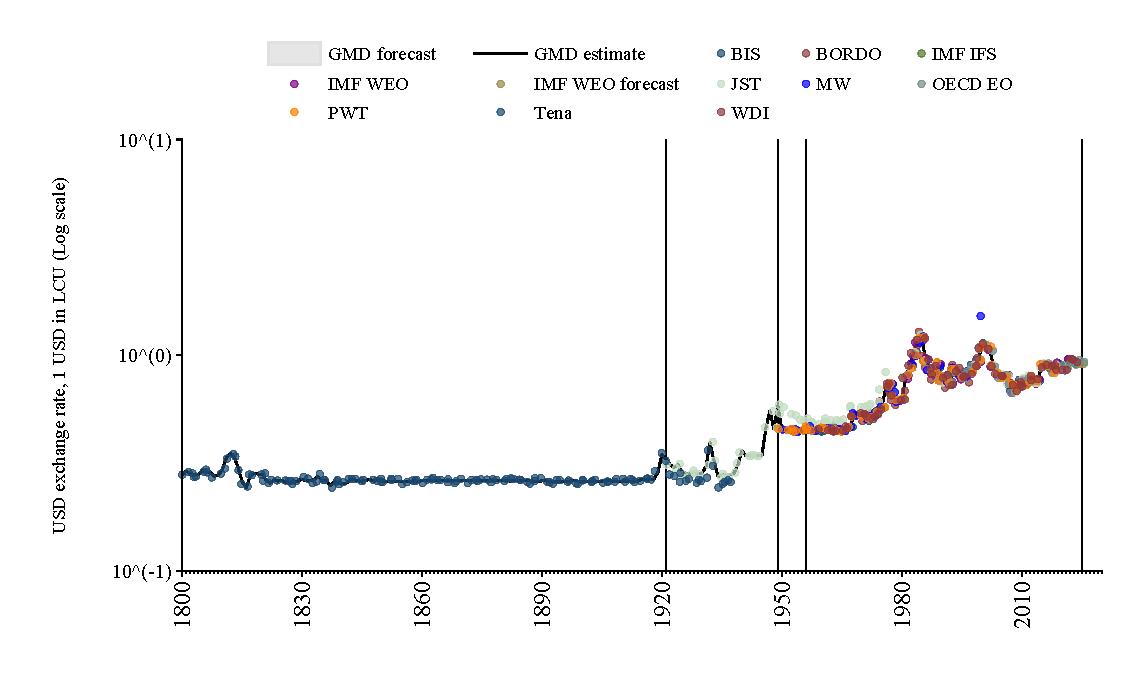
\includegraphics[width=\textwidth,height=0.6\textheight,keepaspectratio]{graphs/IRL_USDfx.pdf}
\end{figure}
\end{minipage}
\end{adjustbox}
\begin{adjustbox}{max totalsize={\paperwidth}{\paperheight},center}
\begin{minipage}[t][\textheight][t]{\textwidth}
\vspace*{0.5cm}
\phantomsection
\addcontentsline{toc}{section}{Central bank policy rate}
\begin{center}
{\Large\bfseries Central bank policy rate}
\end{center}
\vspace{0.5cm}
\begin{table}[H]
\centering
\small
\begin{tabular}{|l|l|l|}
\hline
\textbf{Source} & \textbf{Time span} & \textbf{Notes} \\
\hline
\rowcolor{white}\cite{Homer_Sylla}& 1942 - 1951 &Spliced using overlapping data in 1952. \\
\rowcolor{lightgray}\cite{Grimm}& 1952 - 1954 &Spliced using overlapping data in 1955. \\
\rowcolor{white}\cite{OECD_MEI_ARC}& 1955 - 1971 &Spliced using overlapping data in 1972. \\
\rowcolor{lightgray}\cite{Grimm}& 1972 - 1998 &Spliced using overlapping data in 1999. \\
\rowcolor{white}\cite{OECD_EO}& 1999 - 2012 &Spliced using overlapping data in 2013. \\
\rowcolor{lightgray}\cite{Grimm}& 2013 - 2013 &Spliced using overlapping data in 2014. \\
\rowcolor{white}\cite{OECD_EO}& 2014 - 2025 &Baseline source, overlaps with base year 2018. \\
\hline
\end{tabular}
\end{table}
\begin{figure}[H]
\centering
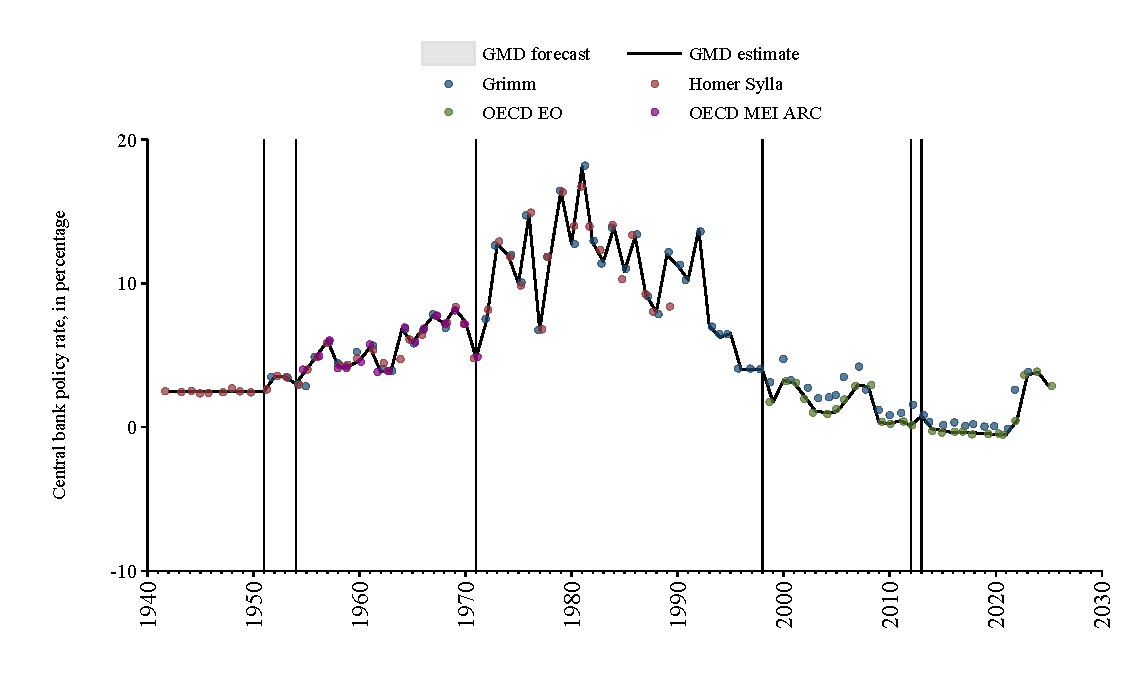
\includegraphics[width=\textwidth,height=0.6\textheight,keepaspectratio]{graphs/IRL_cbrate.pdf}
\end{figure}
\end{minipage}
\end{adjustbox}
\begin{adjustbox}{max totalsize={\paperwidth}{\paperheight},center}
\begin{minipage}[t][\textheight][t]{\textwidth}
\vspace*{0.5cm}
\phantomsection
\addcontentsline{toc}{section}{Total consumption}
\begin{center}
{\Large\bfseries Total consumption}
\end{center}
\vspace{0.5cm}
\begin{table}[H]
\centering
\small
\begin{tabular}{|l|l|l|}
\hline
\textbf{Source} & \textbf{Time span} & \textbf{Notes} \\
\hline
\rowcolor{white}\cite{AMECO}& 1960 - 1989 &Spliced using overlapping data in 1990: (ratio = 99.8\%). \\
\rowcolor{lightgray}\cite{OECD_EO}& 1990 - 2025 &Baseline source, overlaps with base year 2018. \\
\rowcolor{white}\cite{AMECO}& 2026 - 2026 &Spliced using overlapping data in 2027: (ratio = 93.4\%). \\
\hline
\end{tabular}
\end{table}
\begin{figure}[H]
\centering
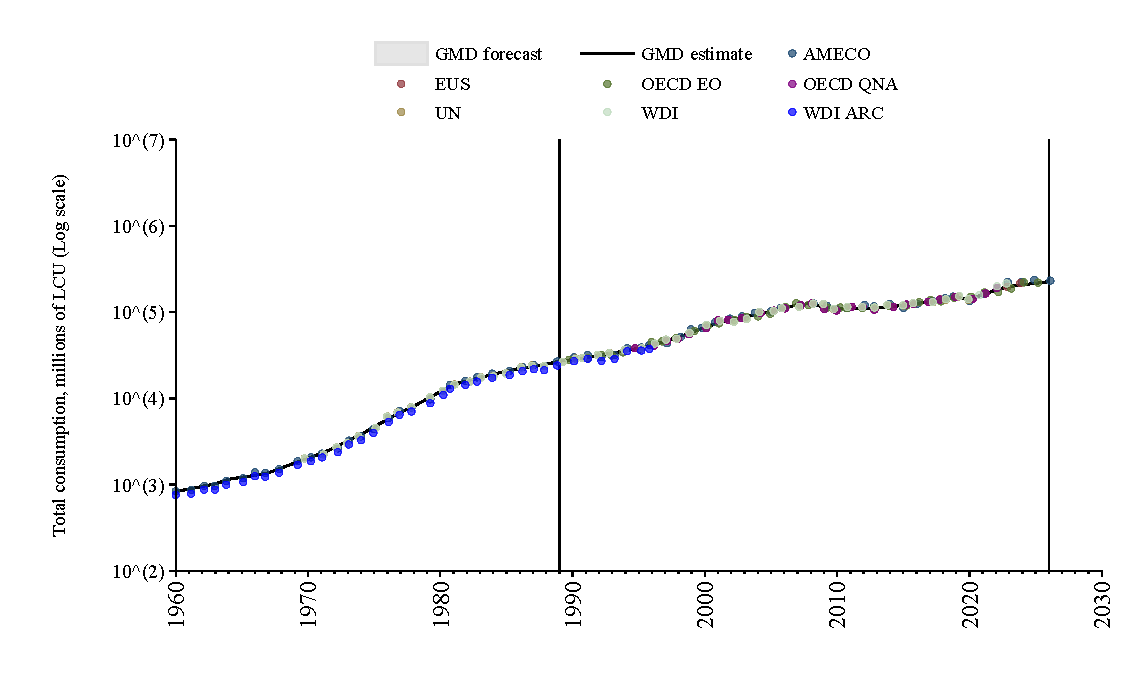
\includegraphics[width=\textwidth,height=0.6\textheight,keepaspectratio]{graphs/IRL_cons.pdf}
\end{figure}
\end{minipage}
\end{adjustbox}
\begin{adjustbox}{max totalsize={\paperwidth}{\paperheight},center}
\begin{minipage}[t][\textheight][t]{\textwidth}
\vspace*{0.5cm}
\phantomsection
\addcontentsline{toc}{section}{Total consumption to GDP ratio}
\begin{center}
{\Large\bfseries Total consumption to GDP ratio}
\end{center}
\vspace{0.5cm}
\begin{table}[H]
\centering
\small
\begin{tabular}{|l|l|l|}
\hline
\textbf{Source} & \textbf{Time span} & \textbf{Notes} \\
\hline
\rowcolor{white}\cite{WDI_ARC}& 1960 - 1969 &Spliced using overlapping data in 1970: (ratio = 101.8\%). \\
\rowcolor{lightgray}\cite{WDI}& 1970 - 2023 &Baseline source, overlaps with base year 2018. \\
\rowcolor{white}\cite{EUS}& 2024 - 2024 &Spliced using overlapping data in 2025. \\
\rowcolor{lightgray}\cite{OECD_EO}& 2025 - 2025 &Spliced using overlapping data in 2026: (ratio = 103.3\%). \\
\rowcolor{white}\cite{AMECO}& 2026 - 2026 &Spliced using overlapping data in 2027: (ratio = 98\%). \\
\hline
\end{tabular}
\end{table}
\begin{figure}[H]
\centering
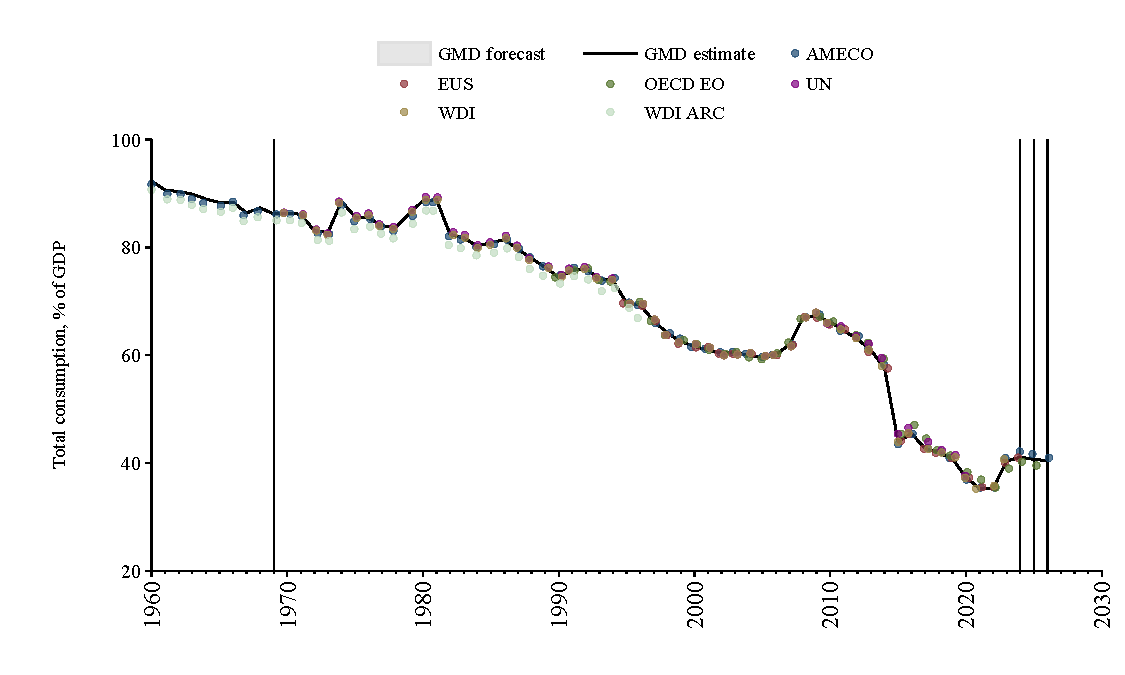
\includegraphics[width=\textwidth,height=0.6\textheight,keepaspectratio]{graphs/IRL_cons_GDP.pdf}
\end{figure}
\end{minipage}
\end{adjustbox}
\begin{adjustbox}{max totalsize={\paperwidth}{\paperheight},center}
\begin{minipage}[t][\textheight][t]{\textwidth}
\vspace*{0.5cm}
\phantomsection
\addcontentsline{toc}{section}{Exports}
\begin{center}
{\Large\bfseries Exports}
\end{center}
\vspace{0.5cm}
\begin{table}[H]
\centering
\small
\begin{tabular}{|l|l|l|}
\hline
\textbf{Source} & \textbf{Time span} & \textbf{Notes} \\
\hline
\rowcolor{white}\cite{Tena}& 1922 - 1937 &Spliced using overlapping data in 1938: (ratio = 106.6\%). \\
\rowcolor{lightgray}\cite{JST}& 1938 - 1959 &Spliced using overlapping data in 1960: (ratio = 100.4\%). \\
\rowcolor{white}\cite{AMECO}& 1960 - 1989 &Spliced using overlapping data in 1990: (ratio = 99.4\%). \\
\rowcolor{lightgray}\cite{OECD_EO}& 1990 - 2025 &Baseline source, overlaps with base year 2018. \\
\rowcolor{white}\cite{AMECO}& 2026 - 2026 &Spliced using overlapping data in 2027: (ratio = 92\%). \\
\rowcolor{lightgray}\cite{IMF_WEO_forecast}& 2027 - 2029 &Spliced using overlapping data in 2030: (ratio = 95.2\%). \\
\hline
\end{tabular}
\end{table}
\begin{figure}[H]
\centering
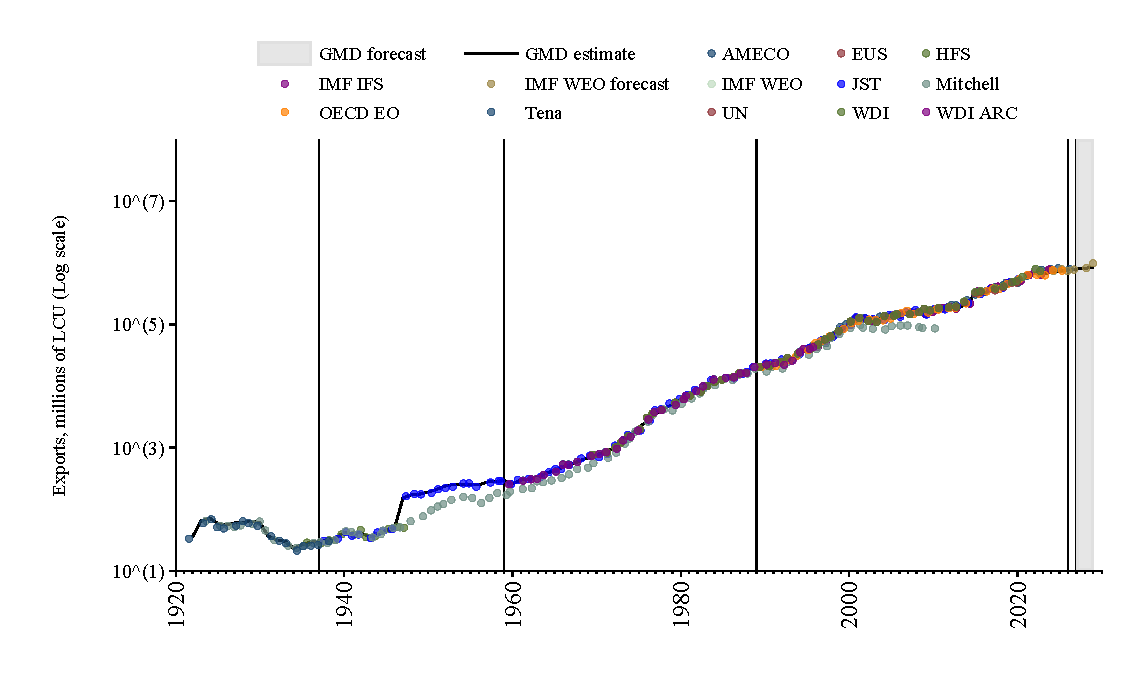
\includegraphics[width=\textwidth,height=0.6\textheight,keepaspectratio]{graphs/IRL_exports.pdf}
\end{figure}
\end{minipage}
\end{adjustbox}
\begin{adjustbox}{max totalsize={\paperwidth}{\paperheight},center}
\begin{minipage}[t][\textheight][t]{\textwidth}
\vspace*{0.5cm}
\phantomsection
\addcontentsline{toc}{section}{Exports to GDP ratio}
\begin{center}
{\Large\bfseries Exports to GDP ratio}
\end{center}
\vspace{0.5cm}
\begin{table}[H]
\centering
\small
\begin{tabular}{|l|l|l|}
\hline
\textbf{Source} & \textbf{Time span} & \textbf{Notes} \\
\hline
\rowcolor{white}\cite{JST}& 1938 - 1969 &Spliced using overlapping data in 1970: (ratio = 100.4\%). \\
\rowcolor{lightgray}\cite{UN}& 1970 - 1989 &Spliced using overlapping data in 1990: (ratio = 99.6\%). \\
\rowcolor{white}\cite{OECD_EO}& 1990 - 2025 &Baseline source, overlaps with base year 2018. \\
\rowcolor{lightgray}\cite{AMECO}& 2026 - 2026 &Spliced using overlapping data in 2027: (ratio = 93.6\%). \\
\rowcolor{white}\cite{IMF_WEO_forecast}& 2027 - 2029 &Spliced using overlapping data in 2030: (ratio = 92.1\%). \\
\hline
\end{tabular}
\end{table}
\begin{figure}[H]
\centering
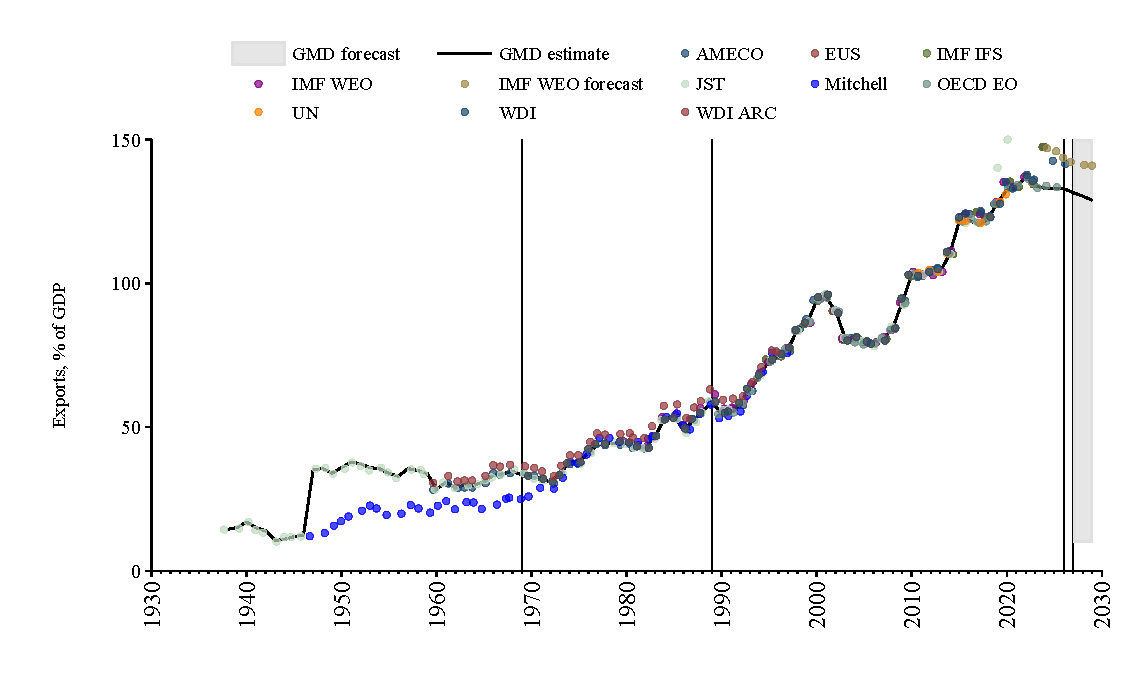
\includegraphics[width=\textwidth,height=0.6\textheight,keepaspectratio]{graphs/IRL_exports_GDP.pdf}
\end{figure}
\end{minipage}
\end{adjustbox}
\begin{adjustbox}{max totalsize={\paperwidth}{\paperheight},center}
\begin{minipage}[t][\textheight][t]{\textwidth}
\vspace*{0.5cm}
\phantomsection
\addcontentsline{toc}{section}{Fixed investment}
\begin{center}
{\Large\bfseries Fixed investment}
\end{center}
\vspace{0.5cm}
\begin{table}[H]
\centering
\small
\begin{tabular}{|l|l|l|}
\hline
\textbf{Source} & \textbf{Time span} & \textbf{Notes} \\
\hline
\rowcolor{white}\cite{AMECO}& 1960 - 1989 &Spliced using overlapping data in 1990: (ratio = 99.5\%). \\
\rowcolor{lightgray}\cite{OECD_EO}& 1990 - 2025 &Baseline source, overlaps with base year 2018. \\
\rowcolor{white}\cite{AMECO}& 2026 - 2026 &Spliced using overlapping data in 2027: (ratio = 105.1\%). \\
\hline
\end{tabular}
\end{table}
\begin{figure}[H]
\centering
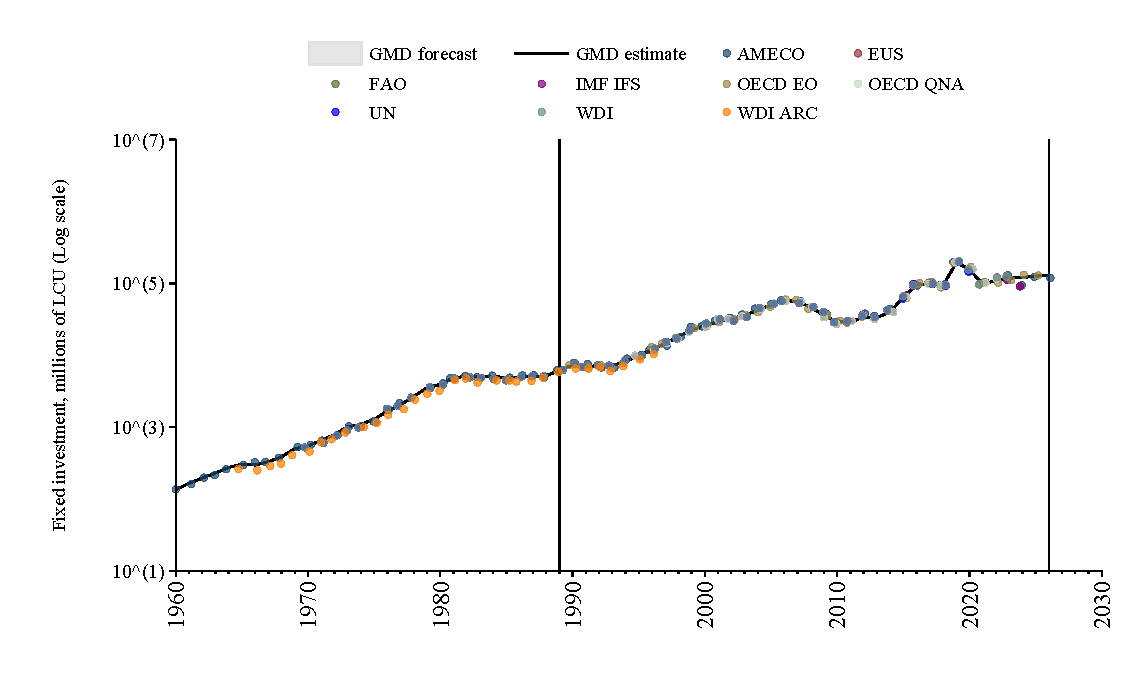
\includegraphics[width=\textwidth,height=0.6\textheight,keepaspectratio]{graphs/IRL_finv.pdf}
\end{figure}
\end{minipage}
\end{adjustbox}
\begin{adjustbox}{max totalsize={\paperwidth}{\paperheight},center}
\begin{minipage}[t][\textheight][t]{\textwidth}
\vspace*{0.5cm}
\phantomsection
\addcontentsline{toc}{section}{Fixed investment to GDP ratio}
\begin{center}
{\Large\bfseries Fixed investment to GDP ratio}
\end{center}
\vspace{0.5cm}
\begin{table}[H]
\centering
\small
\begin{tabular}{|l|l|l|}
\hline
\textbf{Source} & \textbf{Time span} & \textbf{Notes} \\
\hline
\rowcolor{white}\cite{AMECO}& 1960 - 1964 &Spliced using overlapping data in 1965: (ratio = 95.7\%). \\
\rowcolor{lightgray}\cite{WDI_ARC}& 1965 - 1969 &Spliced using overlapping data in 1970: (ratio = 102\%). \\
\rowcolor{white}\cite{WDI}& 1970 - 1994 &Spliced using overlapping data in 1995. \\
\rowcolor{lightgray}\cite{EUS}& 1995 - 2024 &Baseline source, overlaps with base year 2018. \\
\rowcolor{white}\cite{OECD_EO}& 2025 - 2025 &Spliced using overlapping data in 2026: (ratio = 74\%). \\
\rowcolor{lightgray}\cite{AMECO}& 2026 - 2026 &Spliced using overlapping data in 2027: (ratio = 79.1\%). \\
\hline
\end{tabular}
\end{table}
\begin{figure}[H]
\centering
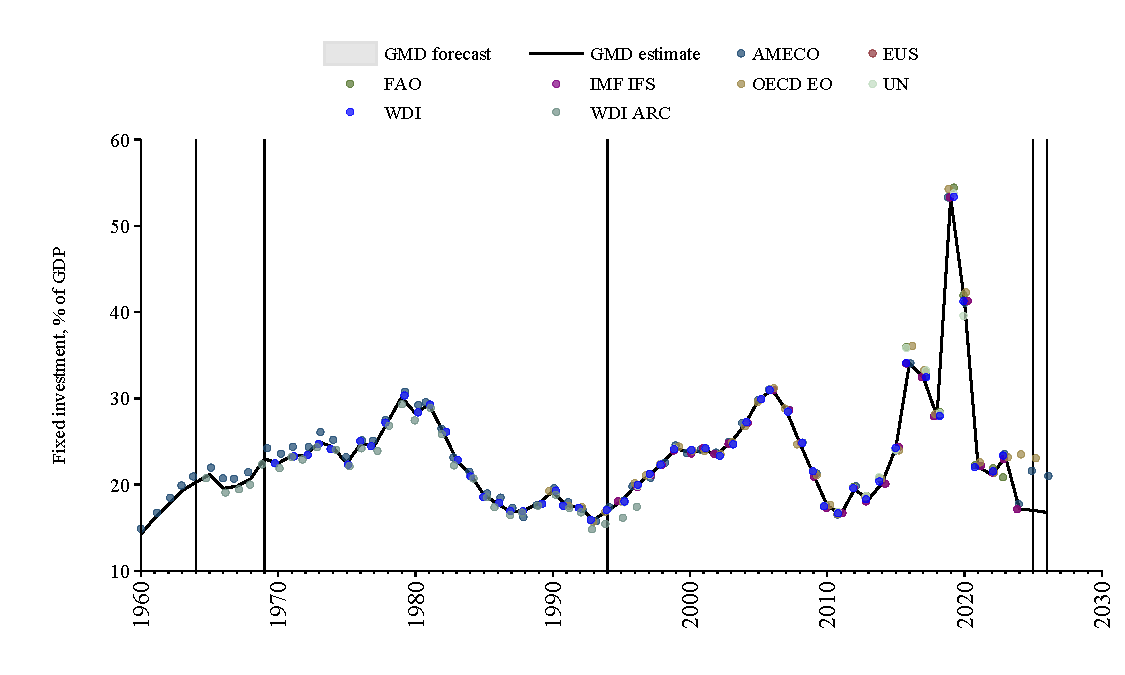
\includegraphics[width=\textwidth,height=0.6\textheight,keepaspectratio]{graphs/IRL_finv_GDP.pdf}
\end{figure}
\end{minipage}
\end{adjustbox}
\begin{adjustbox}{max totalsize={\paperwidth}{\paperheight},center}
\begin{minipage}[t][\textheight][t]{\textwidth}
\vspace*{0.5cm}
\phantomsection
\addcontentsline{toc}{section}{Government debt}
\begin{center}
{\Large\bfseries Government debt}
\end{center}
\vspace{0.5cm}
\begin{table}[H]
\centering
\small
\begin{tabular}{|l|l|l|}
\hline
\textbf{Source} & \textbf{Time span} & \textbf{Notes} \\
\hline
\rowcolor{white}\cite{JST}& 1922 - 1928 &Spliced using overlapping data in 1929. Data refers to both central and general governments.\\
\rowcolor{lightgray}\cite{IMF_FPP}& 1929 - 1929 &Spliced using overlapping data in 1930. Data refers to general government.\\
\rowcolor{white}\cite{JST}& 1930 - 1932 &Spliced using overlapping data in 1933. Data refers to both central and general governments.\\
\rowcolor{lightgray}\cite{IMF_FPP}& 1933 - 1933 &Spliced using overlapping data in 1934. Data refers to general government.\\
\rowcolor{white}\cite{JST}& 1934 - 1935 &Spliced using overlapping data in 1936. Data refers to both central and general governments.\\
\rowcolor{lightgray}\cite{IMF_FPP}& 1936 - 1949 &Spliced using overlapping data in 1950. Data refers to general government.\\
\rowcolor{white}\cite{IMF_GDD}& 1950 - 1993 &Spliced using overlapping data in 1994. Data refers to central government.\\
\rowcolor{lightgray}\cite{IMF_FPP}& 1994 - 1994 &Spliced using overlapping data in 1995. Data refers to general government.\\
\rowcolor{white}\cite{IMF_GDD}& 1995 - 2018 &Spliced using overlapping data in 2019. Data refers to central government.\\
\rowcolor{lightgray}\cite{IMF_FPP}& 2019 - 2023 &Spliced using overlapping data in 2024. Data refers to general government.\\
\rowcolor{white}\cite{OECD_EO}& 2024 - 2025 &Spliced using overlapping data in 2026. Data refers to general government.\\
\rowcolor{lightgray}\cite{IMF_WEO_forecast}& 2026 - 2029 &Spliced using overlapping data in 2030. \\
\hline
\end{tabular}
\end{table}
\begin{figure}[H]
\centering
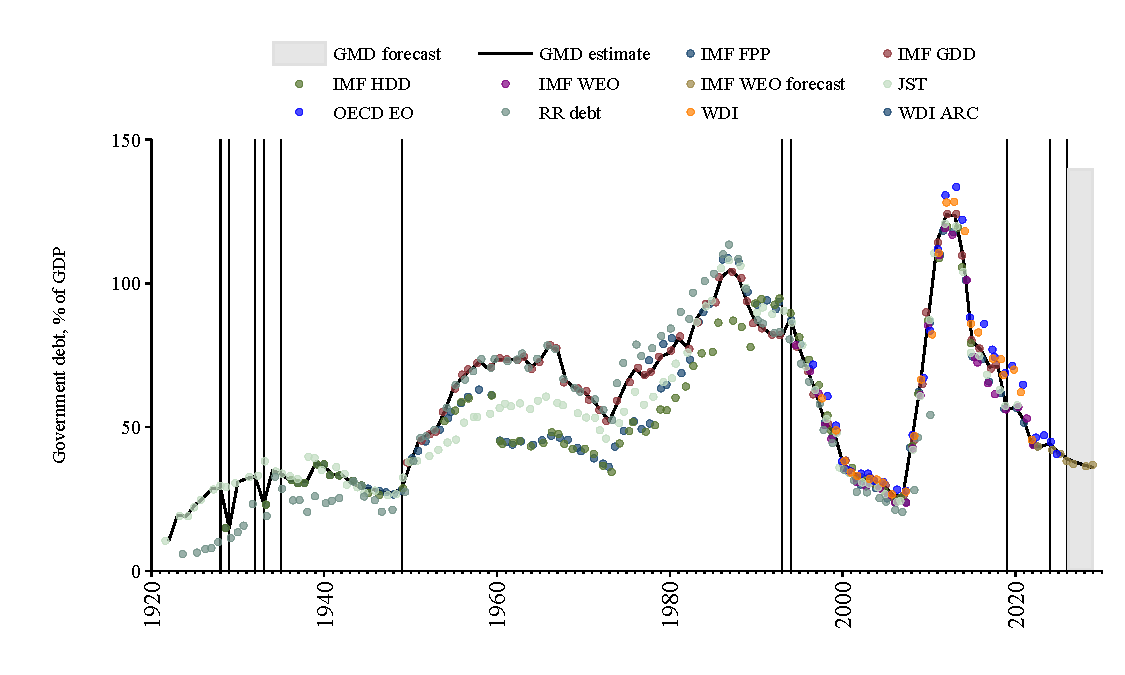
\includegraphics[width=\textwidth,height=0.6\textheight,keepaspectratio]{graphs/IRL_govdebt_GDP.pdf}
\end{figure}
\end{minipage}
\end{adjustbox}
\begin{adjustbox}{max totalsize={\paperwidth}{\paperheight},center}
\begin{minipage}[t][\textheight][t]{\textwidth}
\vspace*{0.5cm}
\phantomsection
\addcontentsline{toc}{section}{Government deficit}
\begin{center}
{\Large\bfseries Government deficit}
\end{center}
\vspace{0.5cm}
\begin{table}[H]
\centering
\small
\begin{tabular}{|l|l|l|}
\hline
\textbf{Source} & \textbf{Time span} & \textbf{Notes} \\
\hline
\rowcolor{white}\cite{IMF_FPP}& 1926 - 1989 &Spliced using overlapping data in 1990. \\
\rowcolor{lightgray}\cite{IMF_GFS}& 1990 - 1994 &Spliced using overlapping data in 1995. \\
\rowcolor{white}\cite{EUS}& 1995 - 2024 &Baseline source, overlaps with base year 2018. \\
\rowcolor{lightgray}\cite{IMF_WEO_forecast}& 2025 - 2029 &Spliced using overlapping data in 2030. \\
\hline
\end{tabular}
\end{table}
\begin{figure}[H]
\centering
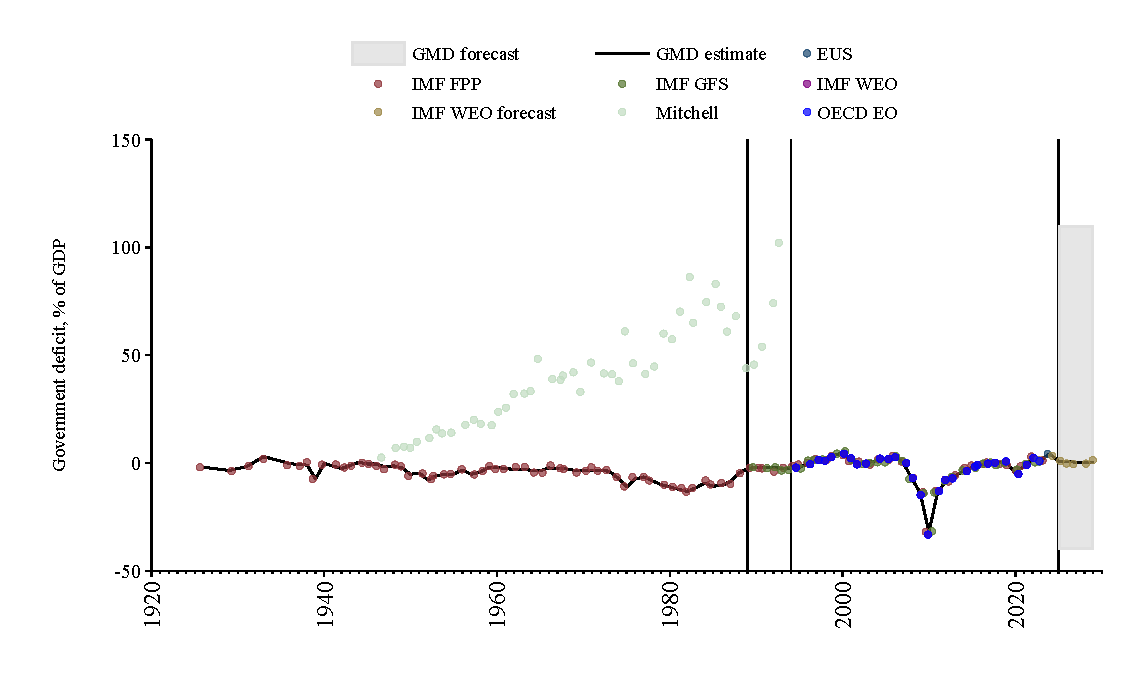
\includegraphics[width=\textwidth,height=0.6\textheight,keepaspectratio]{graphs/IRL_govdef_GDP.pdf}
\end{figure}
\end{minipage}
\end{adjustbox}
\begin{adjustbox}{max totalsize={\paperwidth}{\paperheight},center}
\begin{minipage}[t][\textheight][t]{\textwidth}
\vspace*{0.5cm}
\phantomsection
\addcontentsline{toc}{section}{Government expenditure}
\begin{center}
{\Large\bfseries Government expenditure}
\end{center}
\vspace{0.5cm}
\begin{table}[H]
\centering
\small
\begin{tabular}{|l|l|l|}
\hline
\textbf{Source} & \textbf{Time span} & \textbf{Notes} \\
\hline
\rowcolor{white}\cite{Mitchell}& 1922 - 1925 &Spliced using overlapping data in 1926: (ratio = 104\%). \\
\rowcolor{lightgray}\cite{GMD_estimated}& 1926 - 1926 &Spliced using overlapping data in 1927: (ratio = 119.3\%). \\
\rowcolor{white}\cite{Mitchell}& 1927 - 1928 &Spliced using overlapping data in 1929: (ratio = 104\%). \\
\rowcolor{lightgray}\cite{GMD_estimated}& 1929 - 1929 &Spliced using overlapping data in 1930: (ratio = 114\%). \\
\rowcolor{white}\cite{Mitchell}& 1930 - 1930 &Spliced using overlapping data in 1931: (ratio = 104\%). \\
\rowcolor{lightgray}\cite{GMD_estimated}& 1931 - 1931 &Spliced using overlapping data in 1932: (ratio = 99.3\%). \\
\rowcolor{white}\cite{Mitchell}& 1932 - 1932 &Spliced using overlapping data in 1933: (ratio = 104\%). \\
\rowcolor{lightgray}\cite{GMD_estimated}& 1933 - 1933 &Spliced using overlapping data in 1934: (ratio = 97.1\%). \\
\rowcolor{white}\cite{Mitchell}& 1934 - 1935 &Spliced using overlapping data in 1936: (ratio = 104\%). \\
\rowcolor{lightgray}\cite{GMD_estimated}& 1936 - 2029 &Baseline source, overlaps with base year 2018. \\
\hline
\end{tabular}
\end{table}
\begin{figure}[H]
\centering
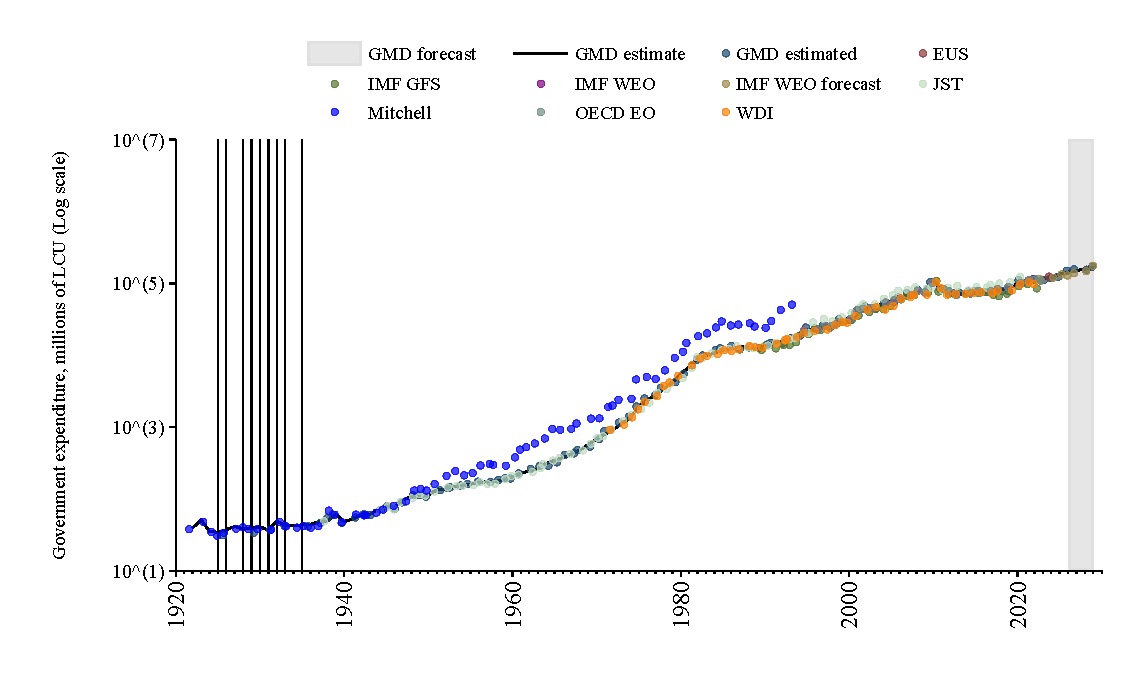
\includegraphics[width=\textwidth,height=0.6\textheight,keepaspectratio]{graphs/IRL_govexp.pdf}
\end{figure}
\end{minipage}
\end{adjustbox}
\begin{adjustbox}{max totalsize={\paperwidth}{\paperheight},center}
\begin{minipage}[t][\textheight][t]{\textwidth}
\vspace*{0.5cm}
\phantomsection
\addcontentsline{toc}{section}{Government expenditure to GDP ratio}
\begin{center}
{\Large\bfseries Government expenditure to GDP ratio}
\end{center}
\vspace{0.5cm}
\begin{table}[H]
\centering
\small
\begin{tabular}{|l|l|l|}
\hline
\textbf{Source} & \textbf{Time span} & \textbf{Notes} \\
\hline
\rowcolor{white}\cite{IMF_FPP}& 1926 - 1937 &Spliced using overlapping data in 1938. Data refers to general government.\\
\rowcolor{lightgray}\cite{JST}& 1938 - 1938 &Spliced using overlapping data in 1939. Data refers to central government.\\
\rowcolor{white}\cite{IMF_FPP}& 1939 - 1943 &Spliced using overlapping data in 1944. Data refers to general government.\\
\rowcolor{lightgray}\cite{JST}& 1944 - 1971 &Spliced using overlapping data in 1972. Data refers to central government.\\
\rowcolor{white}\cite{WDI}& 1972 - 1994 &Spliced using overlapping data in 1995. Data refers to general government.\\
\rowcolor{lightgray}\cite{EUS}& 1995 - 2024 &Baseline source, overlaps with base year 2018. Data refers to general government.\\
\rowcolor{white}\cite{IMF_WEO_forecast}& 2025 - 2029 &Spliced using overlapping data in 2030. \\
\hline
\end{tabular}
\end{table}
\begin{figure}[H]
\centering
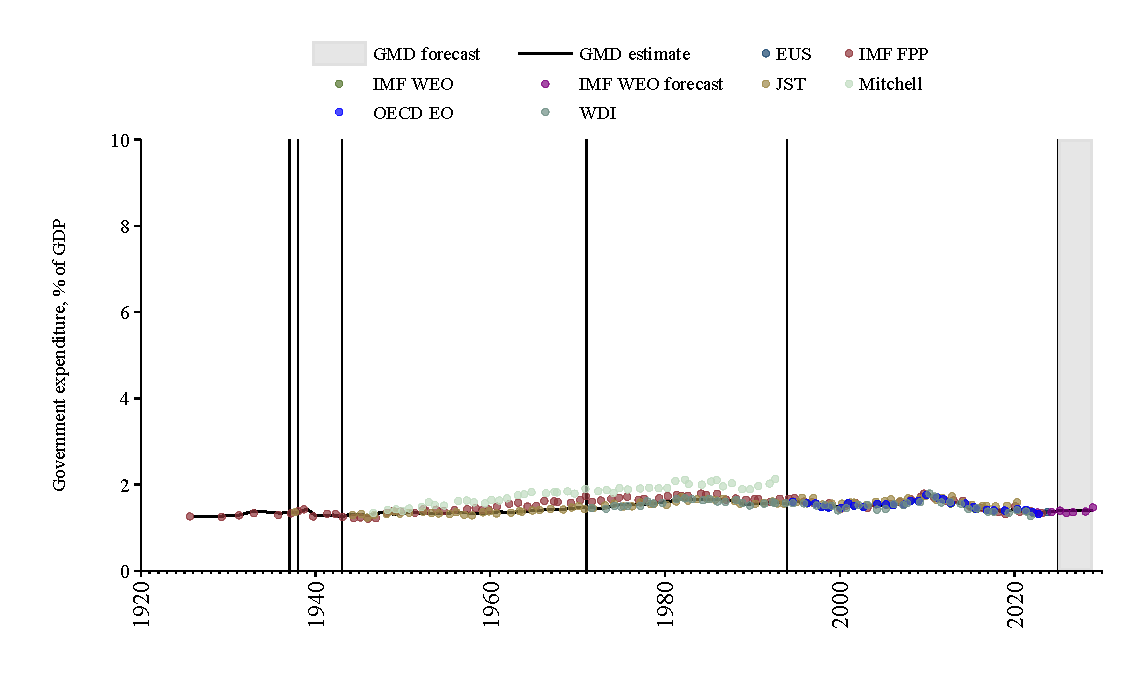
\includegraphics[width=\textwidth,height=0.6\textheight,keepaspectratio]{graphs/IRL_govexp_GDP.pdf}
\end{figure}
\end{minipage}
\end{adjustbox}
\begin{adjustbox}{max totalsize={\paperwidth}{\paperheight},center}
\begin{minipage}[t][\textheight][t]{\textwidth}
\vspace*{0.5cm}
\phantomsection
\addcontentsline{toc}{section}{Government revenue}
\begin{center}
{\Large\bfseries Government revenue}
\end{center}
\vspace{0.5cm}
\begin{table}[H]
\centering
\small
\begin{tabular}{|l|l|l|}
\hline
\textbf{Source} & \textbf{Time span} & \textbf{Notes} \\
\hline
\rowcolor{white}\cite{Mitchell}& 1922 - 1925 &Spliced using overlapping data in 1926: (ratio = 111.3\%). \\
\rowcolor{lightgray}\cite{GMD_estimated}& 1926 - 1926 &Spliced using overlapping data in 1927: (ratio = 126.3\%). \\
\rowcolor{white}\cite{Mitchell}& 1927 - 1928 &Spliced using overlapping data in 1929: (ratio = 111.3\%). \\
\rowcolor{lightgray}\cite{GMD_estimated}& 1929 - 1929 &Spliced using overlapping data in 1930: (ratio = 119.1\%). \\
\rowcolor{white}\cite{Mitchell}& 1930 - 1930 &Spliced using overlapping data in 1931: (ratio = 111.3\%). \\
\rowcolor{lightgray}\cite{GMD_estimated}& 1931 - 1931 &Spliced using overlapping data in 1932: (ratio = 104.2\%). \\
\rowcolor{white}\cite{Mitchell}& 1932 - 1932 &Spliced using overlapping data in 1933: (ratio = 111.3\%). \\
\rowcolor{lightgray}\cite{GMD_estimated}& 1933 - 1933 &Spliced using overlapping data in 1934: (ratio = 84.4\%). \\
\rowcolor{white}\cite{Mitchell}& 1934 - 1935 &Spliced using overlapping data in 1936: (ratio = 111.3\%). \\
\rowcolor{lightgray}\cite{GMD_estimated}& 1936 - 2029 &Baseline source, overlaps with base year 2018. \\
\hline
\end{tabular}
\end{table}
\begin{figure}[H]
\centering
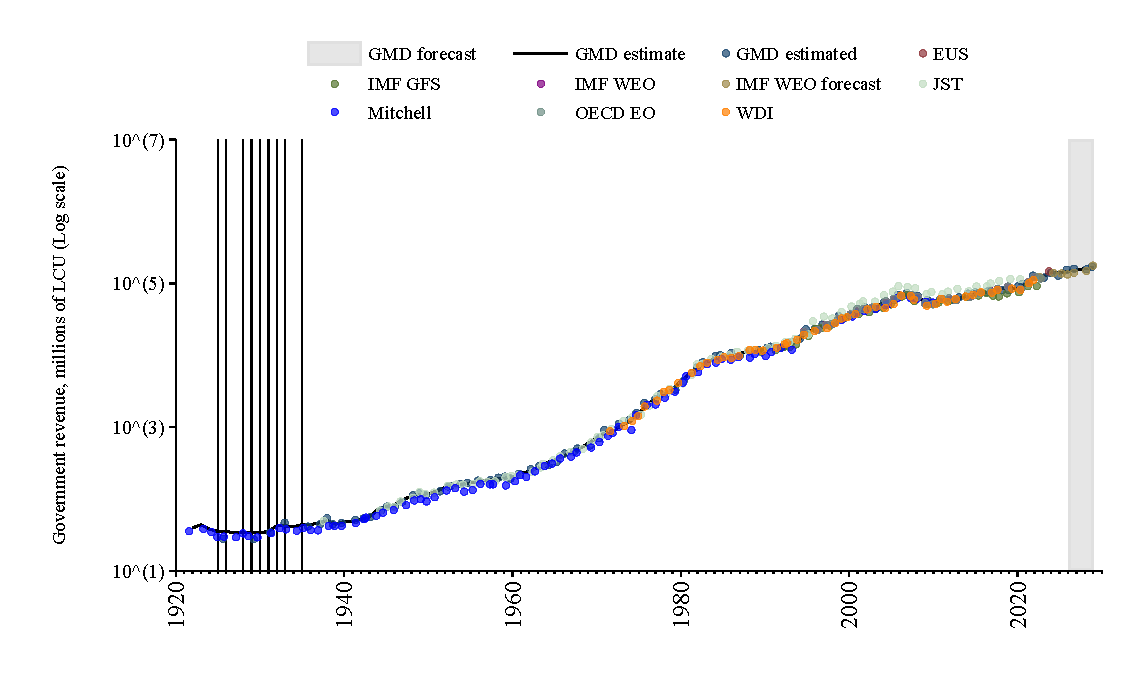
\includegraphics[width=\textwidth,height=0.6\textheight,keepaspectratio]{graphs/IRL_govrev.pdf}
\end{figure}
\end{minipage}
\end{adjustbox}
\begin{adjustbox}{max totalsize={\paperwidth}{\paperheight},center}
\begin{minipage}[t][\textheight][t]{\textwidth}
\vspace*{0.5cm}
\phantomsection
\addcontentsline{toc}{section}{Government revenue to GDP ratio}
\begin{center}
{\Large\bfseries Government revenue to GDP ratio}
\end{center}
\vspace{0.5cm}
\begin{table}[H]
\centering
\small
\begin{tabular}{|l|l|l|}
\hline
\textbf{Source} & \textbf{Time span} & \textbf{Notes} \\
\hline
\rowcolor{white}\cite{IMF_FPP}& 1926 - 1937 &Spliced using overlapping data in 1938. Data refers to general government.\\
\rowcolor{lightgray}\cite{JST}& 1938 - 1938 &Spliced using overlapping data in 1939. Data refers to central government.\\
\rowcolor{white}\cite{IMF_FPP}& 1939 - 1943 &Spliced using overlapping data in 1944. Data refers to general government.\\
\rowcolor{lightgray}\cite{JST}& 1944 - 1971 &Spliced using overlapping data in 1972. Data refers to central government.\\
\rowcolor{white}\cite{WDI}& 1972 - 1994 &Spliced using overlapping data in 1995. Data refers to general government.\\
\rowcolor{lightgray}\cite{OECD_EO}& 1995 - 2023 &Baseline source, overlaps with base year 2018. Data refers to general government.\\
\rowcolor{white}\cite{EUS}& 2024 - 2024 &Spliced using overlapping data in 2025. Data refers to general government.\\
\rowcolor{lightgray}\cite{IMF_WEO_forecast}& 2025 - 2029 &Spliced using overlapping data in 2030. \\
\hline
\end{tabular}
\end{table}
\begin{figure}[H]
\centering
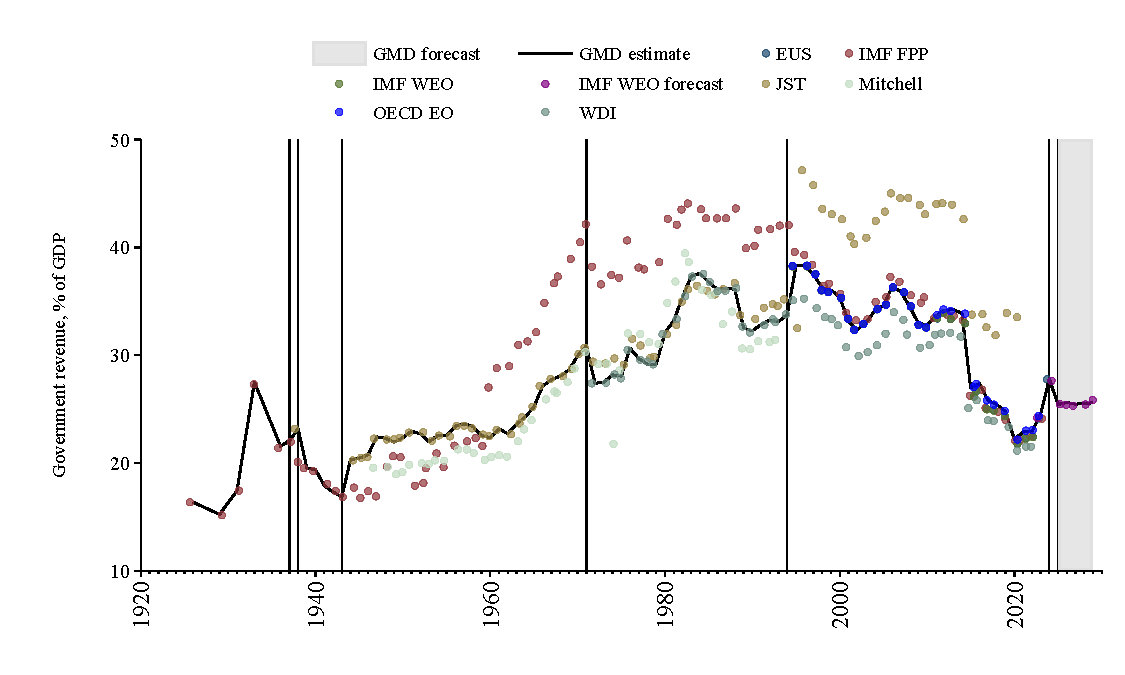
\includegraphics[width=\textwidth,height=0.6\textheight,keepaspectratio]{graphs/IRL_govrev_GDP.pdf}
\end{figure}
\end{minipage}
\end{adjustbox}
\begin{adjustbox}{max totalsize={\paperwidth}{\paperheight},center}
\begin{minipage}[t][\textheight][t]{\textwidth}
\vspace*{0.5cm}
\phantomsection
\addcontentsline{toc}{section}{Government tax revenue}
\begin{center}
{\Large\bfseries Government tax revenue}
\end{center}
\vspace{0.5cm}
\begin{table}[H]
\centering
\small
\begin{tabular}{|l|l|l|}
\hline
\textbf{Source} & \textbf{Time span} & \textbf{Notes} \\
\hline
\rowcolor{white}\cite{Mitchell}& 1922 - 1946 &Spliced using overlapping data in 1947. \\
\rowcolor{lightgray}\cite{GMD_estimated}& 1947 - 2023 &Baseline source, overlaps with base year 2018. \\
\hline
\end{tabular}
\end{table}
\begin{figure}[H]
\centering
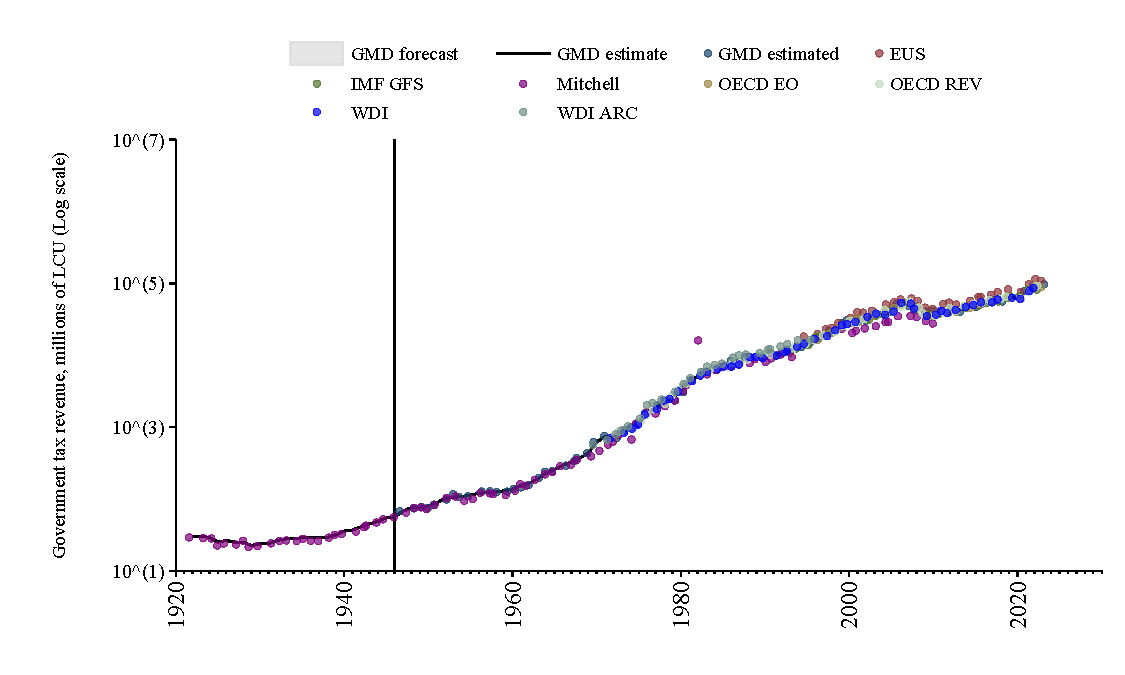
\includegraphics[width=\textwidth,height=0.6\textheight,keepaspectratio]{graphs/IRL_govtax.pdf}
\end{figure}
\end{minipage}
\end{adjustbox}
\begin{adjustbox}{max totalsize={\paperwidth}{\paperheight},center}
\begin{minipage}[t][\textheight][t]{\textwidth}
\vspace*{0.5cm}
\phantomsection
\addcontentsline{toc}{section}{Government tax revenue to GDP ratio}
\begin{center}
{\Large\bfseries Government tax revenue to GDP ratio}
\end{center}
\vspace{0.5cm}
\begin{table}[H]
\centering
\small
\begin{tabular}{|l|l|l|}
\hline
\textbf{Source} & \textbf{Time span} & \textbf{Notes} \\
\hline
\rowcolor{white}\cite{Mitchell}& 1947 - 1969 &Spliced using overlapping data in 1970. Data refers to central government.\\
\rowcolor{lightgray}\cite{WDI_ARC}& 1970 - 1971 &Spliced using overlapping data in 1972. Data refers to central government.\\
\rowcolor{white}\cite{WDI}& 1972 - 1994 &Spliced using overlapping data in 1995. Data refers to central government.\\
\rowcolor{lightgray}\cite{OECD_EO}& 1995 - 2023 &Baseline source, overlaps with base year 2018. Data refers to general government.\\
\hline
\end{tabular}
\end{table}
\begin{figure}[H]
\centering
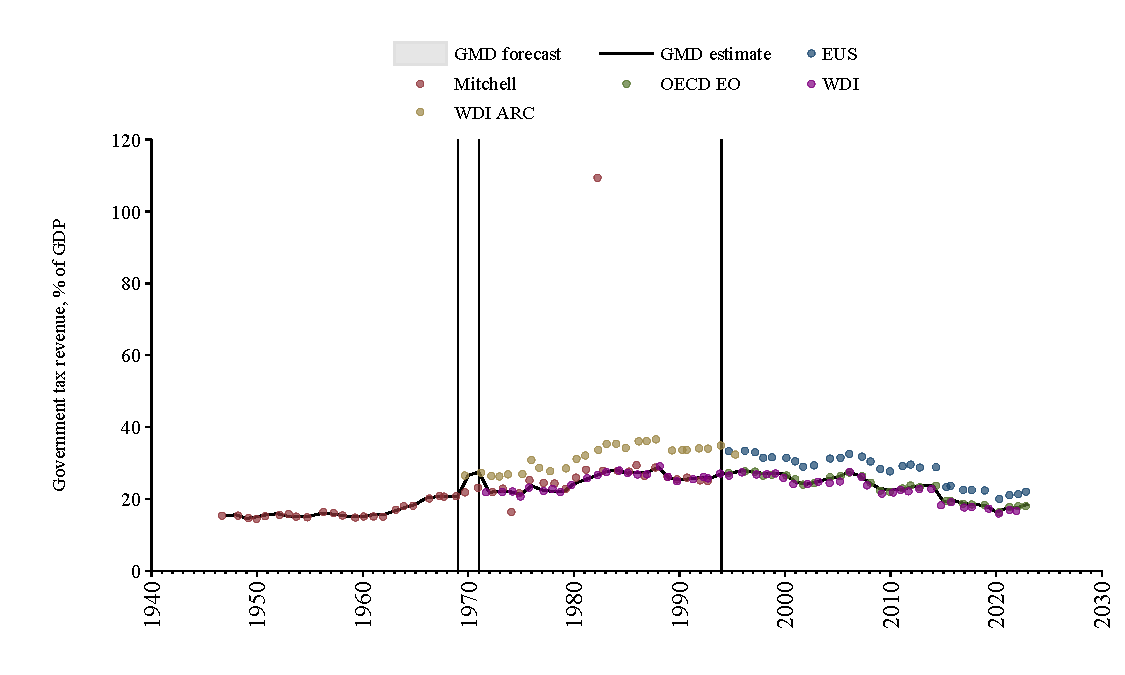
\includegraphics[width=\textwidth,height=0.6\textheight,keepaspectratio]{graphs/IRL_govtax_GDP.pdf}
\end{figure}
\end{minipage}
\end{adjustbox}
\begin{adjustbox}{max totalsize={\paperwidth}{\paperheight},center}
\begin{minipage}[t][\textheight][t]{\textwidth}
\vspace*{0.5cm}
\phantomsection
\addcontentsline{toc}{section}{Imports}
\begin{center}
{\Large\bfseries Imports}
\end{center}
\vspace{0.5cm}
\begin{table}[H]
\centering
\small
\begin{tabular}{|l|l|l|}
\hline
\textbf{Source} & \textbf{Time span} & \textbf{Notes} \\
\hline
\rowcolor{white}\cite{Tena}& 1922 - 1937 &Spliced using overlapping data in 1938: (ratio = 109\%). \\
\rowcolor{lightgray}\cite{JST}& 1938 - 1959 &Spliced using overlapping data in 1960: (ratio = 103.2\%). \\
\rowcolor{white}\cite{AMECO}& 1960 - 1989 &Spliced using overlapping data in 1990. \\
\rowcolor{lightgray}\cite{OECD_EO}& 1990 - 2025 &Baseline source, overlaps with base year 2018. \\
\rowcolor{white}\cite{AMECO}& 2026 - 2026 &Spliced using overlapping data in 2027: (ratio = 91.8\%). \\
\rowcolor{lightgray}\cite{IMF_WEO_forecast}& 2027 - 2029 &Spliced using overlapping data in 2030: (ratio = 95.8\%). \\
\hline
\end{tabular}
\end{table}
\begin{figure}[H]
\centering
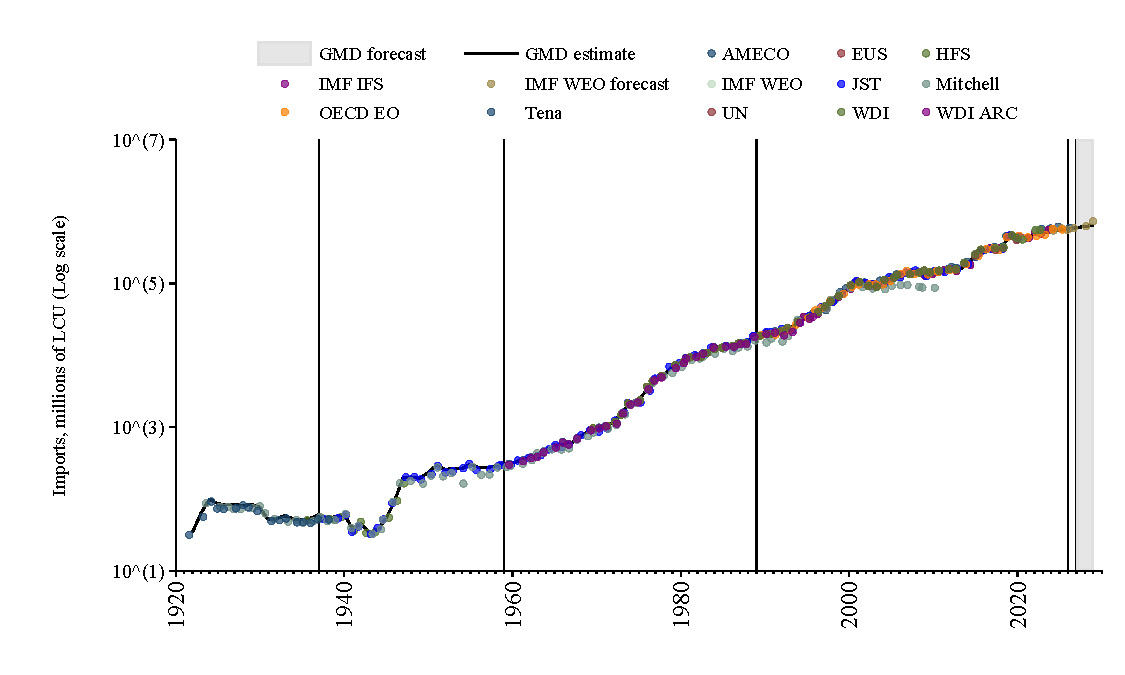
\includegraphics[width=\textwidth,height=0.6\textheight,keepaspectratio]{graphs/IRL_imports.pdf}
\end{figure}
\end{minipage}
\end{adjustbox}
\begin{adjustbox}{max totalsize={\paperwidth}{\paperheight},center}
\begin{minipage}[t][\textheight][t]{\textwidth}
\vspace*{0.5cm}
\phantomsection
\addcontentsline{toc}{section}{Imports to GDP ratio}
\begin{center}
{\Large\bfseries Imports to GDP ratio}
\end{center}
\vspace{0.5cm}
\begin{table}[H]
\centering
\small
\begin{tabular}{|l|l|l|}
\hline
\textbf{Source} & \textbf{Time span} & \textbf{Notes} \\
\hline
\rowcolor{white}\cite{JST}& 1938 - 1959 &Spliced using overlapping data in 1960: (ratio = 103.7\%). \\
\rowcolor{lightgray}\cite{WDI_ARC}& 1960 - 1969 &Spliced using overlapping data in 1970: (ratio = 95.5\%). \\
\rowcolor{white}\cite{WDI}& 1970 - 1989 &Spliced using overlapping data in 1990: (ratio = 100.2\%). \\
\rowcolor{lightgray}\cite{OECD_EO}& 1990 - 2025 &Baseline source, overlaps with base year 2018. \\
\rowcolor{white}\cite{AMECO}& 2026 - 2026 &Spliced using overlapping data in 2027: (ratio = 93.3\%). \\
\rowcolor{lightgray}\cite{IMF_WEO_forecast}& 2027 - 2029 &Spliced using overlapping data in 2030: (ratio = 92.7\%). \\
\hline
\end{tabular}
\end{table}
\begin{figure}[H]
\centering
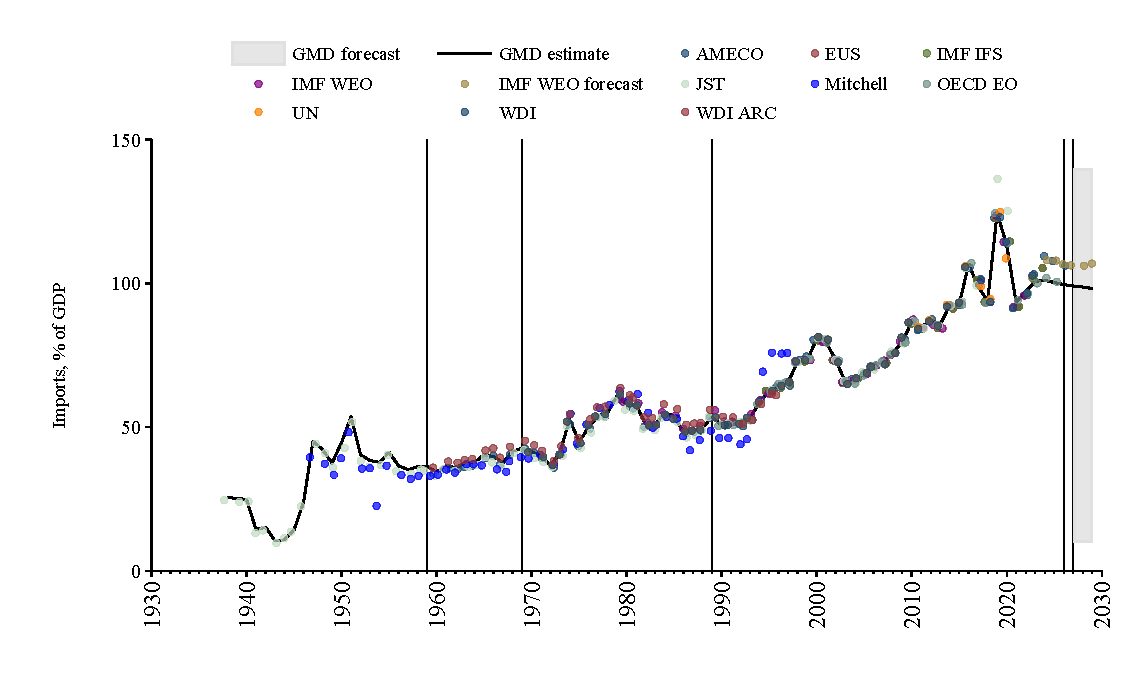
\includegraphics[width=\textwidth,height=0.6\textheight,keepaspectratio]{graphs/IRL_imports_GDP.pdf}
\end{figure}
\end{minipage}
\end{adjustbox}
\begin{adjustbox}{max totalsize={\paperwidth}{\paperheight},center}
\begin{minipage}[t][\textheight][t]{\textwidth}
\vspace*{0.5cm}
\phantomsection
\addcontentsline{toc}{section}{Inflation}
\begin{center}
{\Large\bfseries Inflation}
\end{center}
\vspace{0.5cm}
\begin{table}[H]
\centering
\small
\begin{tabular}{|l|l|l|}
\hline
\textbf{Source} & \textbf{Time span} & \textbf{Notes} \\
\hline
\rowcolor{white}\cite{CLIO}& 1922 - 1922 &Spliced using overlapping data in 1923. \\
\rowcolor{lightgray}\cite{BIS}& 1923 - 1969 &Spliced using overlapping data in 1970. \\
\rowcolor{white}\cite{WB_CC}& 1970 - 1995 &Spliced using overlapping data in 1996. \\
\rowcolor{lightgray}\cite{OECD_EO}& 1996 - 2025 &Baseline source, overlaps with base year 2018. \\
\rowcolor{white}\cite{IMF_WEO_forecast}& 2026 - 2029 &Spliced using overlapping data in 2030. \\
\hline
\end{tabular}
\end{table}
\begin{figure}[H]
\centering
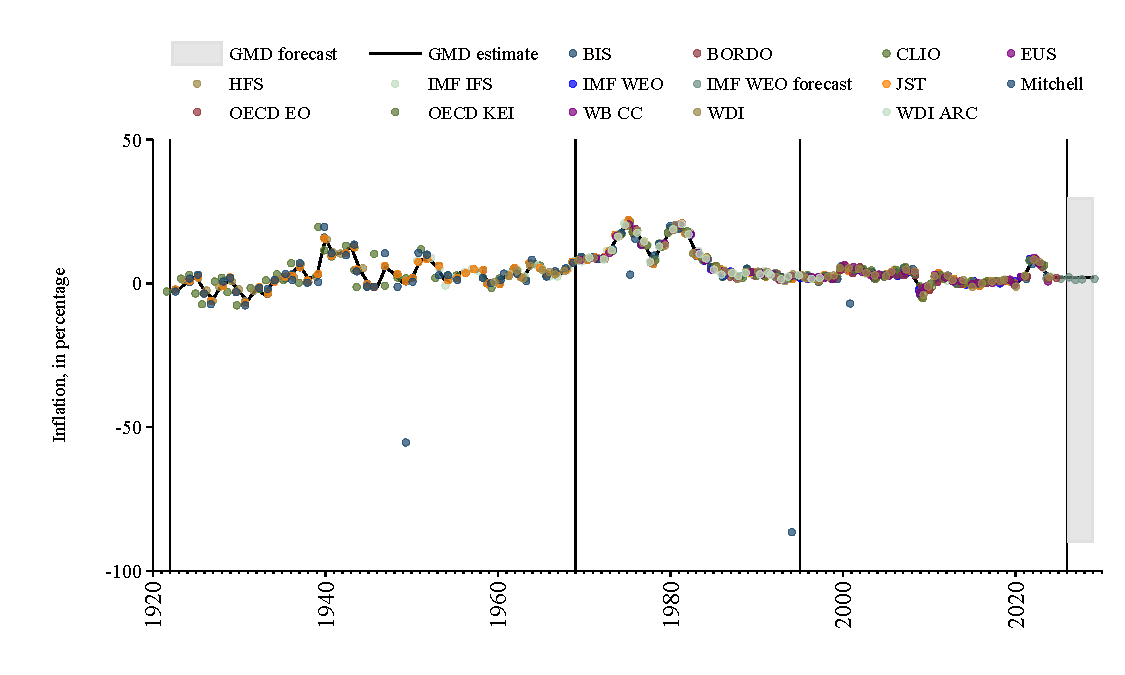
\includegraphics[width=\textwidth,height=0.6\textheight,keepaspectratio]{graphs/IRL_infl.pdf}
\end{figure}
\end{minipage}
\end{adjustbox}
\begin{adjustbox}{max totalsize={\paperwidth}{\paperheight},center}
\begin{minipage}[t][\textheight][t]{\textwidth}
\vspace*{0.5cm}
\phantomsection
\addcontentsline{toc}{section}{Investment}
\begin{center}
{\Large\bfseries Investment}
\end{center}
\vspace{0.5cm}
\begin{table}[H]
\centering
\small
\begin{tabular}{|l|l|l|}
\hline
\textbf{Source} & \textbf{Time span} & \textbf{Notes} \\
\hline
\rowcolor{white}\cite{JST}& 1938 - 1959 &Spliced using overlapping data in 1960: (ratio = 103\%). \\
\rowcolor{lightgray}\cite{AMECO}& 1960 - 1989 &Spliced using overlapping data in 1990: (ratio = 99.6\%). \\
\rowcolor{white}\cite{OECD_EO}& 1990 - 2025 &Baseline source, overlaps with base year 2018. \\
\rowcolor{lightgray}\cite{AMECO}& 2026 - 2026 &Spliced using overlapping data in 2027: (ratio = 117\%). \\
\rowcolor{white}\cite{IMF_WEO_forecast}& 2027 - 2029 &Spliced using overlapping data in 2030: (ratio = 152.7\%). \\
\hline
\end{tabular}
\end{table}
\begin{figure}[H]
\centering
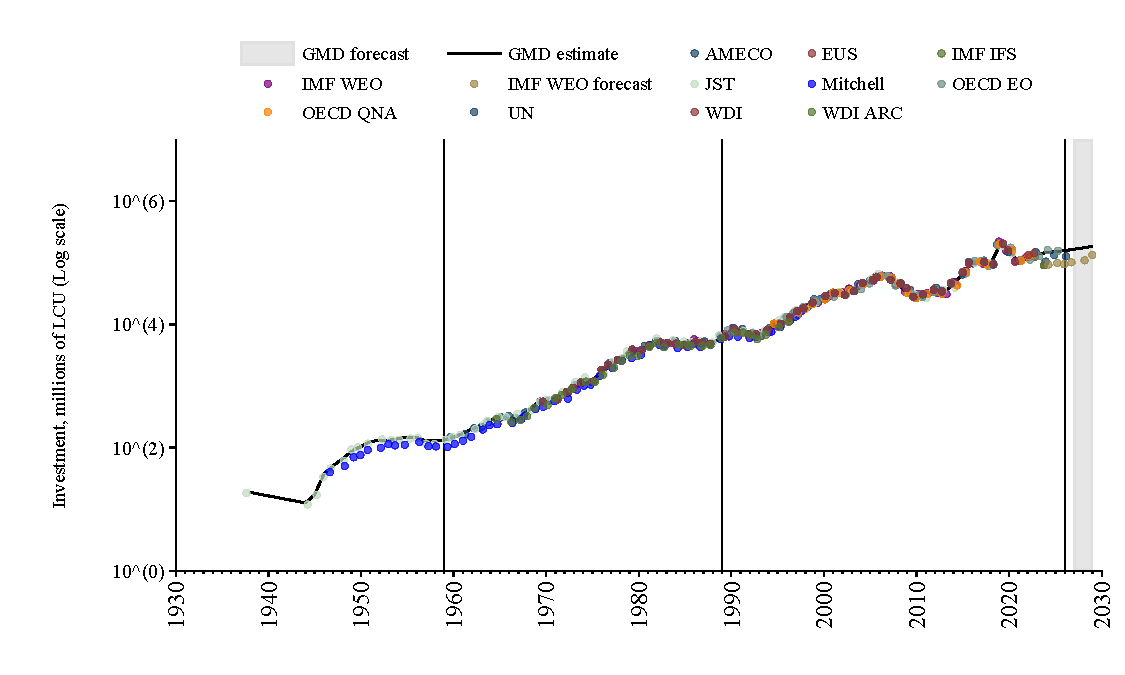
\includegraphics[width=\textwidth,height=0.6\textheight,keepaspectratio]{graphs/IRL_inv.pdf}
\end{figure}
\end{minipage}
\end{adjustbox}
\begin{adjustbox}{max totalsize={\paperwidth}{\paperheight},center}
\begin{minipage}[t][\textheight][t]{\textwidth}
\vspace*{0.5cm}
\phantomsection
\addcontentsline{toc}{section}{Investment to GDP ratio}
\begin{center}
{\Large\bfseries Investment to GDP ratio}
\end{center}
\vspace{0.5cm}
\begin{table}[H]
\centering
\small
\begin{tabular}{|l|l|l|}
\hline
\textbf{Source} & \textbf{Time span} & \textbf{Notes} \\
\hline
\rowcolor{white}\cite{JST}& 1938 - 1959 &Spliced using overlapping data in 1960: (ratio = 101.9\%). \\
\rowcolor{lightgray}\cite{AMECO}& 1960 - 1964 &Spliced using overlapping data in 1965: (ratio = 99.8\%). \\
\rowcolor{white}\cite{WDI_ARC}& 1965 - 1969 &Spliced using overlapping data in 1970: (ratio = 101.2\%). \\
\rowcolor{lightgray}\cite{WDI}& 1970 - 1989 &Spliced using overlapping data in 1990: (ratio = 99.9\%). \\
\rowcolor{white}\cite{OECD_EO}& 1990 - 2025 &Baseline source, overlaps with base year 2018. \\
\rowcolor{lightgray}\cite{AMECO}& 2026 - 2026 &Spliced using overlapping data in 2027: (ratio = 119\%). \\
\rowcolor{white}\cite{IMF_WEO_forecast}& 2027 - 2029 &Spliced using overlapping data in 2030: (ratio = 147.7\%). \\
\hline
\end{tabular}
\end{table}
\begin{figure}[H]
\centering
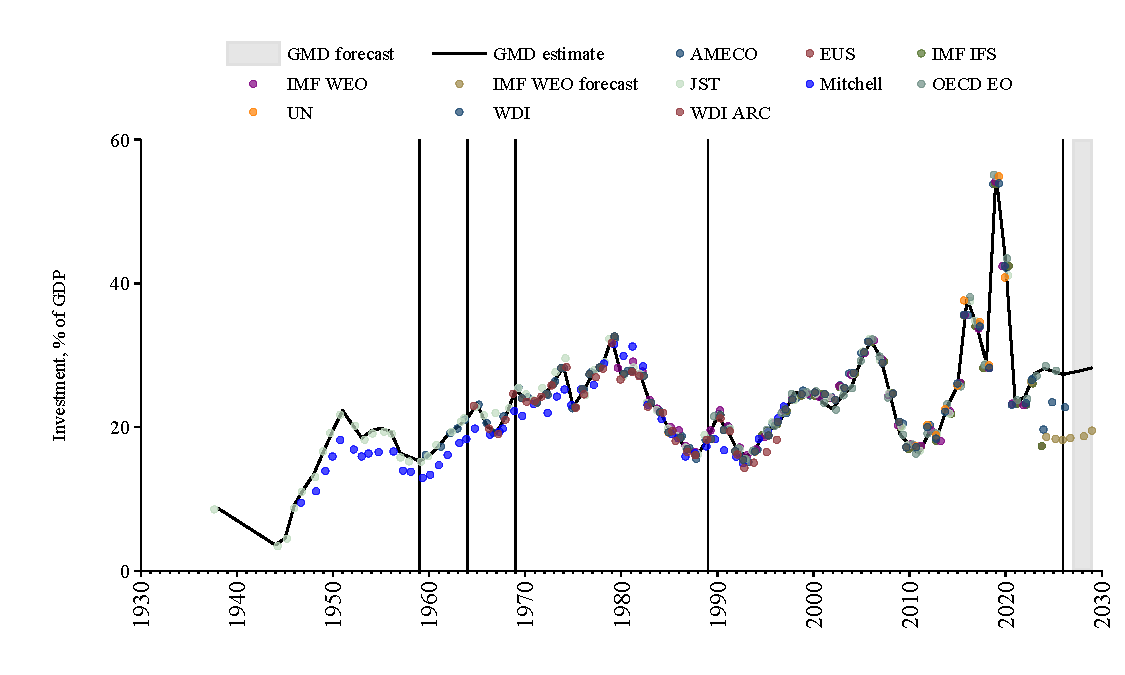
\includegraphics[width=\textwidth,height=0.6\textheight,keepaspectratio]{graphs/IRL_inv_GDP.pdf}
\end{figure}
\end{minipage}
\end{adjustbox}
\begin{adjustbox}{max totalsize={\paperwidth}{\paperheight},center}
\begin{minipage}[t][\textheight][t]{\textwidth}
\vspace*{0.5cm}
\phantomsection
\addcontentsline{toc}{section}{Long term interest rate}
\begin{center}
{\Large\bfseries Long term interest rate}
\end{center}
\vspace{0.5cm}
\begin{table}[H]
\centering
\small
\begin{tabular}{|l|l|l|}
\hline
\textbf{Source} & \textbf{Time span} & \textbf{Notes} \\
\hline
\rowcolor{white}\cite{JST}& 1922 - 1970 &Spliced using overlapping data in 1971. \\
\rowcolor{lightgray}\cite{OECD_MEI}& 1971 - 2023 &Baseline source, overlaps with base year 2018. \\
\rowcolor{white}\cite{EUS}& 2024 - 2024 &Spliced using overlapping data in 2025. \\
\hline
\end{tabular}
\end{table}
\begin{figure}[H]
\centering
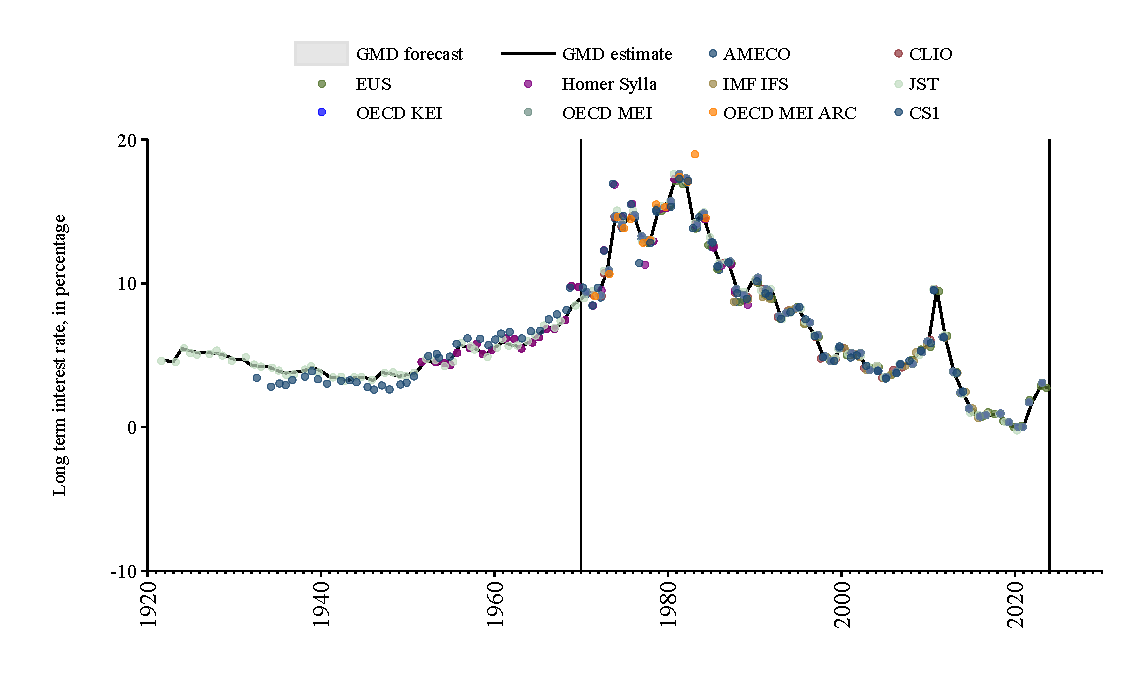
\includegraphics[width=\textwidth,height=0.6\textheight,keepaspectratio]{graphs/IRL_ltrate.pdf}
\end{figure}
\end{minipage}
\end{adjustbox}
\begin{adjustbox}{max totalsize={\paperwidth}{\paperheight},center}
\begin{minipage}[t][\textheight][t]{\textwidth}
\vspace*{0.5cm}
\phantomsection
\addcontentsline{toc}{section}{Nominal GDP}
\begin{center}
{\Large\bfseries Nominal GDP}
\end{center}
\vspace{0.5cm}
\begin{table}[H]
\centering
\small
\begin{tabular}{|l|l|l|}
\hline
\textbf{Source} & \textbf{Time span} & \textbf{Notes} \\
\hline
\rowcolor{white}\cite{HFS}& 1861 - 1920 &Spliced using overlapping data in 1921: (ratio = 105.2\%). \\
\rowcolor{lightgray}\cite{JST}& 1921 - 1932 &Spliced using overlapping data in 1933: (ratio = 102.5\%). \\
\rowcolor{white}\cite{CS1_IRL}& 1933 - 1949 &Spliced using overlapping data in 1950: (ratio = 2331.1\%). \\
\rowcolor{lightgray}\cite{IMF_GDD}& 1950 - 1959 &Spliced using overlapping data in 1960: (ratio = 100.1\%). \\
\rowcolor{white}\cite{AMECO}& 1960 - 1989 &Spliced using overlapping data in 1990: (ratio = 99.8\%). \\
\rowcolor{lightgray}\cite{OECD_EO}& 1990 - 2025 &Baseline source, overlaps with base year 2018. \\
\rowcolor{white}\cite{AMECO}& 2026 - 2026 &Spliced using overlapping data in 2027: (ratio = 98.4\%). \\
\rowcolor{lightgray}\cite{IMF_WEO_forecast}& 2027 - 2029 &Spliced using overlapping data in 2030: (ratio = 103.4\%). \\
\hline
\end{tabular}
\end{table}
\begin{figure}[H]
\centering
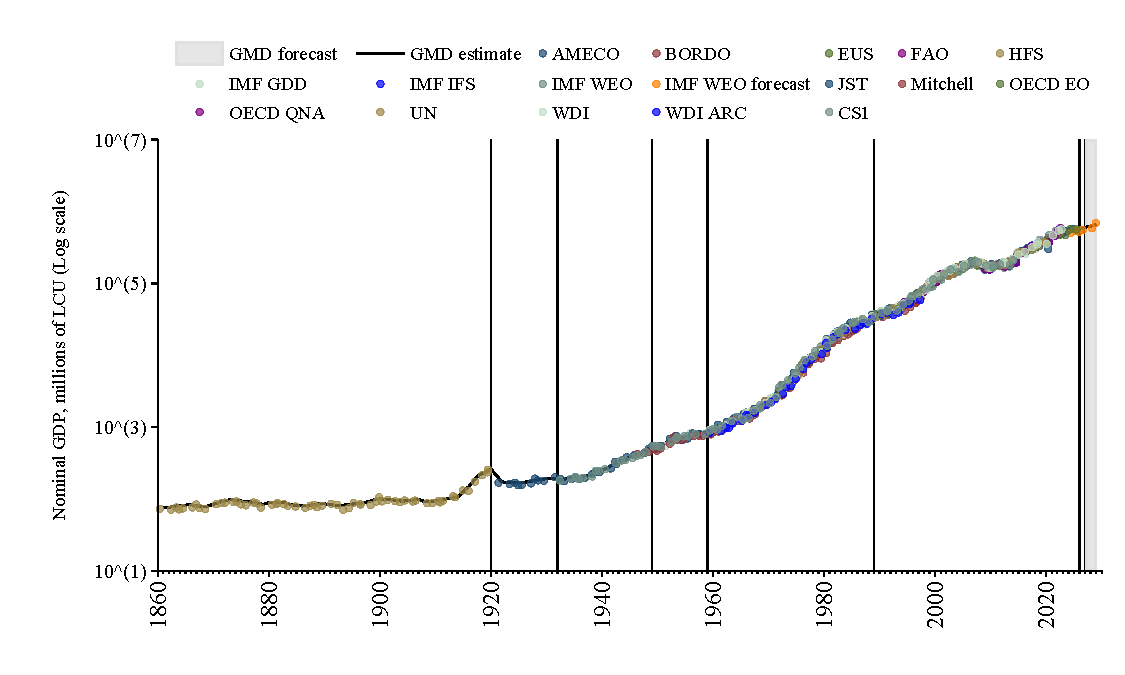
\includegraphics[width=\textwidth,height=0.6\textheight,keepaspectratio]{graphs/IRL_nGDP.pdf}
\end{figure}
\end{minipage}
\end{adjustbox}
\begin{adjustbox}{max totalsize={\paperwidth}{\paperheight},center}
\begin{minipage}[t][\textheight][t]{\textwidth}
\vspace*{0.5cm}
\phantomsection
\addcontentsline{toc}{section}{Population}
\begin{center}
{\Large\bfseries Population}
\end{center}
\vspace{0.5cm}
\begin{table}[H]
\centering
\small
\begin{tabular}{|l|l|l|}
\hline
\textbf{Source} & \textbf{Time span} & \textbf{Notes} \\
\hline
\rowcolor{white}\cite{Gapminder}& 1800 - 1949 &Spliced using overlapping data in 1950: (ratio = 101.4\%). \\
\rowcolor{lightgray}\cite{IMF_IFS}& 1950 - 1959 &Spliced using overlapping data in 1960: (ratio = 101.3\%). \\
\rowcolor{white}\cite{WDI}& 1960 - 2023 &Baseline source, overlaps with base year 2018. \\
\rowcolor{lightgray}\cite{OECD_EO}& 2024 - 2025 &Spliced using overlapping data in 2026: (ratio = 102.6\%). \\
\rowcolor{white}\cite{AMECO}& 2026 - 2026 &Spliced using overlapping data in 2027: (ratio = 98.7\%). \\
\rowcolor{lightgray}\cite{Gapminder}& 2027 - 2030 &Spliced using overlapping data in 2031: (ratio = 101.5\%). \\
\hline
\end{tabular}
\end{table}
\begin{figure}[H]
\centering
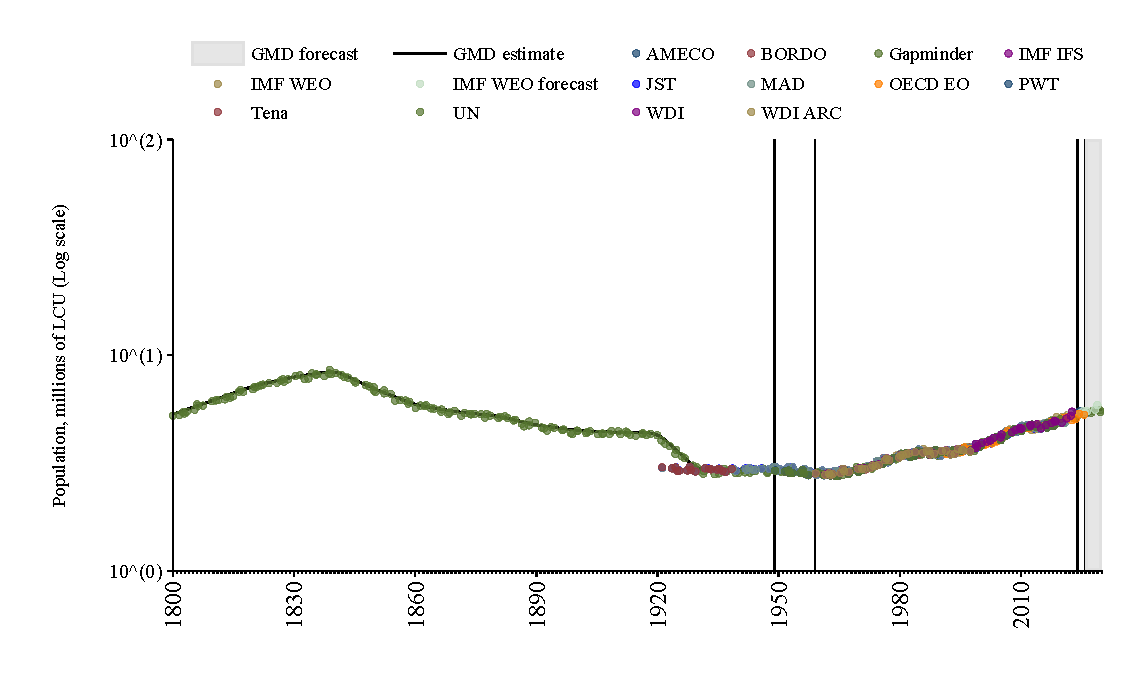
\includegraphics[width=\textwidth,height=0.6\textheight,keepaspectratio]{graphs/IRL_pop.pdf}
\end{figure}
\end{minipage}
\end{adjustbox}
\begin{adjustbox}{max totalsize={\paperwidth}{\paperheight},center}
\begin{minipage}[t][\textheight][t]{\textwidth}
\vspace*{0.5cm}
\phantomsection
\addcontentsline{toc}{section}{Real GDP}
\begin{center}
{\Large\bfseries Real GDP}
\end{center}
\vspace{0.5cm}
\begin{table}[H]
\centering
\small
\begin{tabular}{|l|l|l|}
\hline
\textbf{Source} & \textbf{Time span} & \textbf{Notes} \\
\hline
\rowcolor{white}\cite{JST}& 1922 - 1932 &Spliced using overlapping data in 1933: (ratio = 35165.4\%). \\
\rowcolor{lightgray}\cite{CS1_IRL}& 1933 - 1959 &Spliced using overlapping data in 1960: (ratio = 27691\%). \\
\rowcolor{white}\cite{AMECO}& 1960 - 1989 &Spliced using overlapping data in 1990: (ratio = 101.6\%). \\
\rowcolor{lightgray}\cite{OECD_EO}& 1990 - 2025 &Baseline source, overlaps with base year 2018. \\
\rowcolor{white}\cite{AMECO}& 2026 - 2026 &Spliced using overlapping data in 2027. \\
\rowcolor{lightgray}\cite{IMF_WEO_forecast}& 2027 - 2029 &Spliced using overlapping data in 2030: (ratio = 102.5\%). \\
\hline
\end{tabular}
\end{table}
\begin{figure}[H]
\centering
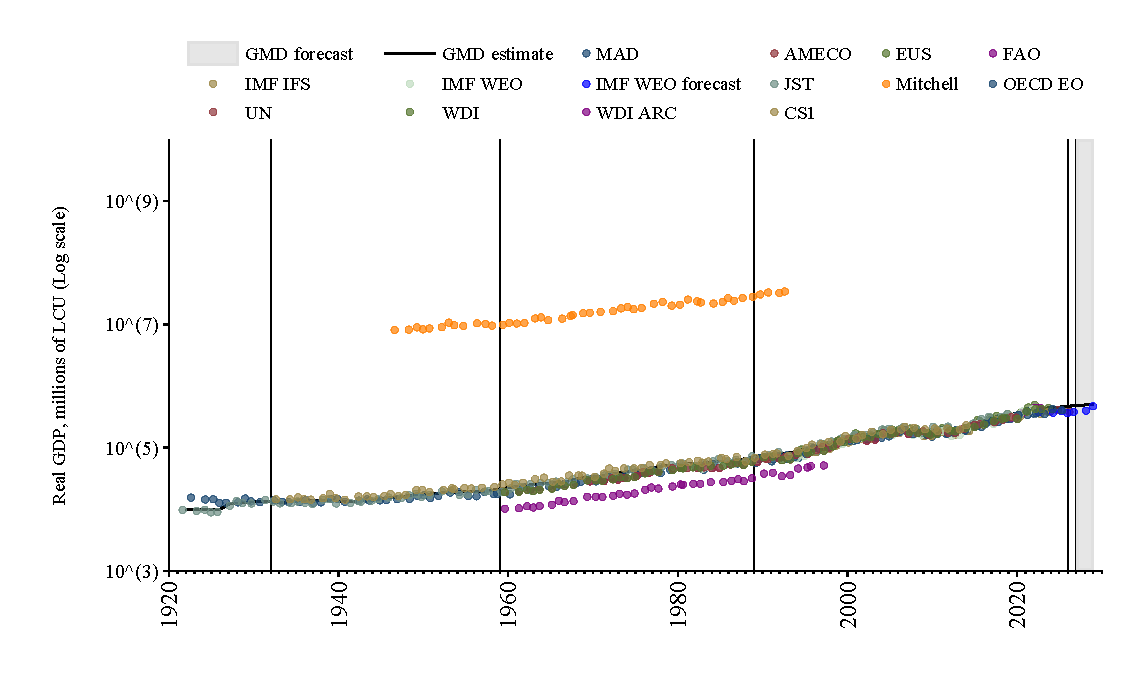
\includegraphics[width=\textwidth,height=0.6\textheight,keepaspectratio]{graphs/IRL_rGDP.pdf}
\end{figure}
\end{minipage}
\end{adjustbox}
\begin{adjustbox}{max totalsize={\paperwidth}{\paperheight},center}
\begin{minipage}[t][\textheight][t]{\textwidth}
\vspace*{0.5cm}
\phantomsection
\addcontentsline{toc}{section}{Real total consumption}
\begin{center}
{\Large\bfseries Real total consumption}
\end{center}
\vspace{0.5cm}
\begin{table}[H]
\centering
\small
\begin{tabular}{|l|l|l|}
\hline
\textbf{Source} & \textbf{Time span} & \textbf{Notes} \\
\hline
\rowcolor{white}\cite{WDI}& 1970 - 1994 &Spliced using overlapping data in 1995. \\
\rowcolor{lightgray}\cite{IMF_IFS}& 1995 - 2024 &Baseline source, overlaps with base year 2018. \\
\hline
\end{tabular}
\end{table}
\begin{figure}[H]
\centering
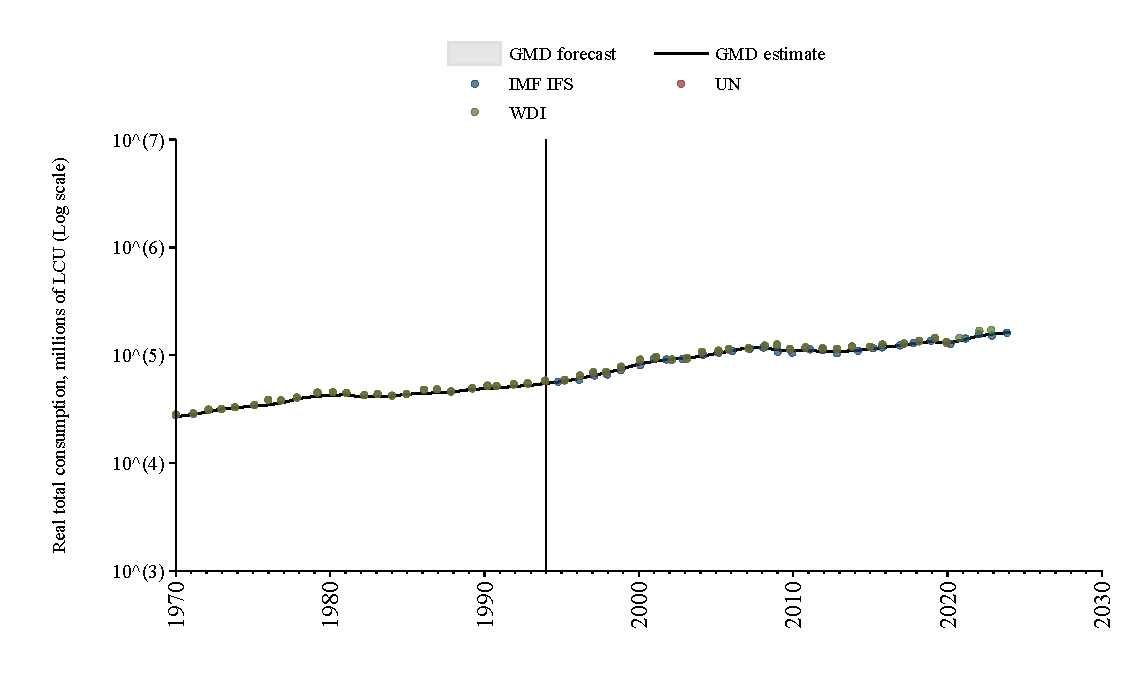
\includegraphics[width=\textwidth,height=0.6\textheight,keepaspectratio]{graphs/IRL_rcons.pdf}
\end{figure}
\end{minipage}
\end{adjustbox}
\begin{adjustbox}{max totalsize={\paperwidth}{\paperheight},center}
\begin{minipage}[t][\textheight][t]{\textwidth}
\vspace*{0.5cm}
\phantomsection
\addcontentsline{toc}{section}{Short term interest rate}
\begin{center}
{\Large\bfseries Short term interest rate}
\end{center}
\vspace{0.5cm}
\begin{table}[H]
\centering
\small
\begin{tabular}{|l|l|l|}
\hline
\textbf{Source} & \textbf{Time span} & \textbf{Notes} \\
\hline
\rowcolor{white}\cite{JST}& 1922 - 1932 &Spliced using overlapping data in 1933. \\
\rowcolor{lightgray}\cite{CS1_IRL}& 1933 - 1970 &Spliced using overlapping data in 1971. \\
\rowcolor{white}\cite{AMECO}& 1971 - 1971 &Spliced using overlapping data in 1972. \\
\rowcolor{lightgray}\cite{OECD_MEI_ARC}& 1972 - 1983 &Spliced using overlapping data in 1984. \\
\rowcolor{white}\cite{OECD_KEI}& 1984 - 2023 &Baseline source, overlaps with base year 2018. \\
\rowcolor{lightgray}\cite{OECD_EO}& 2024 - 2025 &Spliced using overlapping data in 2026. \\
\hline
\end{tabular}
\end{table}
\begin{figure}[H]
\centering
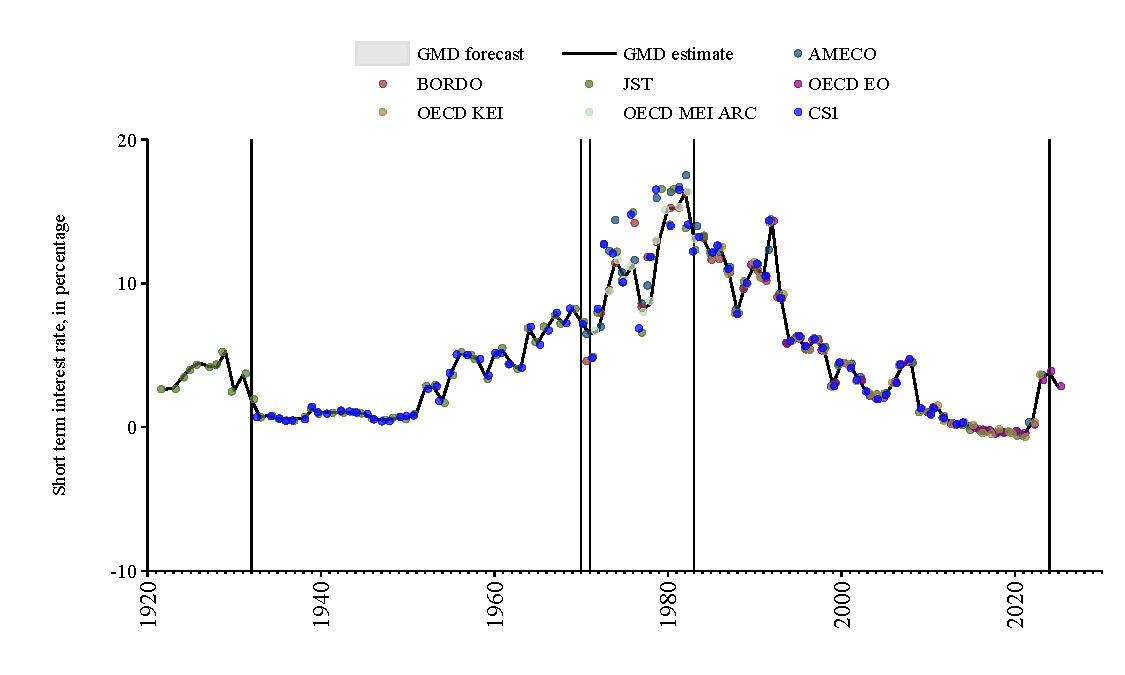
\includegraphics[width=\textwidth,height=0.6\textheight,keepaspectratio]{graphs/IRL_strate.pdf}
\end{figure}
\end{minipage}
\end{adjustbox}
\begin{adjustbox}{max totalsize={\paperwidth}{\paperheight},center}
\begin{minipage}[t][\textheight][t]{\textwidth}
\vspace*{0.5cm}
\phantomsection
\addcontentsline{toc}{section}{Unemployment}
\begin{center}
{\Large\bfseries Unemployment}
\end{center}
\vspace{0.5cm}
\begin{table}[H]
\centering
\small
\begin{tabular}{|l|l|l|}
\hline
\textbf{Source} & \textbf{Time span} & \textbf{Notes} \\
\hline
\rowcolor{white}\cite{CS1_IRL}& 1933 - 1959 &Spliced using overlapping data in 1960. \\
\rowcolor{lightgray}\cite{AMECO}& 1960 - 1982 &Spliced using overlapping data in 1983. \\
\rowcolor{white}\cite{OECD_KEI}& 1983 - 1989 &Spliced using overlapping data in 1990. \\
\rowcolor{lightgray}\cite{OECD_EO}& 1990 - 2008 &Spliced using overlapping data in 2009. \\
\rowcolor{white}\cite{EUS}& 2009 - 2024 &Baseline source, overlaps with base year 2018. \\
\rowcolor{lightgray}\cite{OECD_EO}& 2025 - 2025 &Spliced using overlapping data in 2026. \\
\rowcolor{white}\cite{AMECO}& 2026 - 2026 &Spliced using overlapping data in 2027. \\
\rowcolor{lightgray}\cite{IMF_WEO_forecast}& 2027 - 2029 &Spliced using overlapping data in 2030. \\
\hline
\end{tabular}
\end{table}
\begin{figure}[H]
\centering
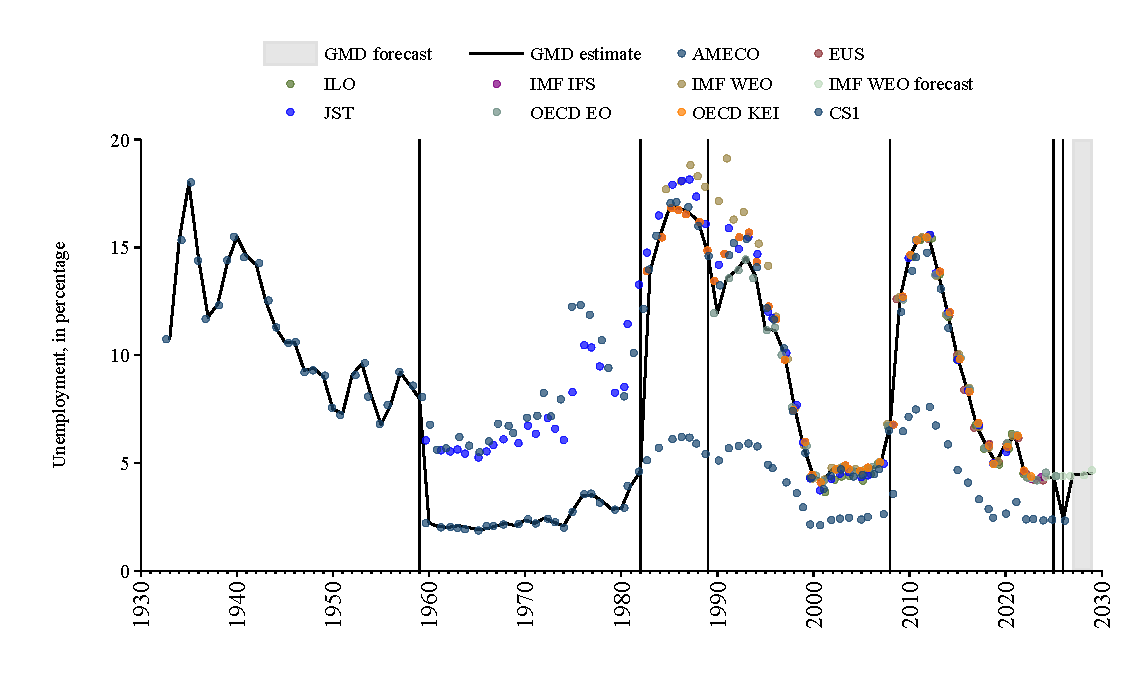
\includegraphics[width=\textwidth,height=0.6\textheight,keepaspectratio]{graphs/IRL_unemp.pdf}
\end{figure}
\end{minipage}
\end{adjustbox}
\phantomsection
\addcontentsline{toc}{section}{References}
\begin{center}
{\Large\bfseries References}
\end{center}
\small
\bibliographystyle{qje}
\bibliography{bib}
\end{document}
